% EE2000 mid-term report, team 22.  Progress report built on the preliminary report (PPR-22).
% Colour rule: black = stated, planned or cited in the PPR (including PPR plans now carried out);
%              blue  = new ideas, new literature, and the mathematics, calculations and numerical results worked out since the PPR.
\documentclass[10pt,twocolumn,letterpaper]{article}

\usepackage[review]{cvpr}      % review version, as for the preliminary report

\usepackage{graphicx}
\usepackage{amsmath}
\usepackage{amssymb}
\usepackage{booktabs}
\usepackage{multirow}
\usepackage{array}
\usepackage{xcolor}
\usepackage{tikz}
\usetikzlibrary{arrows.meta,positioning,calc}

\usepackage[pagebackref,breaklinks,colorlinks]{hyperref}
\usepackage[capitalize]{cleveref}
\crefname{section}{Sec.}{Secs.}
\Crefname{section}{Section}{Sections}
\Crefname{table}{Table}{Tables}
\crefname{table}{Tab.}{Tabs.}
\crefname{appendix}{App.}{Apps.}

% ---------------------------------------------------------------- new content is blue
\newcommand{\nb}[1]{{\color{blue}#1}}
\newenvironment{newtext}{\par\color{blue}}{\par}
\newcommand{\lvl}[1]{\textup{#1}}   % validation level label (L1 ... L5)

\def\cvprPaperID{22}
\def\confName{EE2000}
\def\confYear{2026}

\raggedbottom
\begin{document}

\title{FPGA-Based LMS Tracking of Time-Varying ISI Channels:\\
How Fast Can a Channel Change Before a Fixed-Point Equalizer Loses It?\\
{\large Mid-Term Progress Report}}

\author{Team 22}
\maketitle

%%%%%%%%% ABSTRACT
\begin{abstract}
When an inter-symbol interference (ISI) channel changes with time, the optimum equalizer becomes a moving target. This project asks how fast that target may move before a fixed-point least mean squares (LMS) equalizer, intended for an FPGA, can no longer follow it. A baseband BPSK link with a deliberately time-varying channel feeds three receivers on one impaired stream: a direct detector, an LMS equalizer trained once and frozen, and a continuously adapting LMS equalizer. Bit-error rate, mean-square error and reacquisition time are measured against the variation rate, the step size and the coefficient word length. This mid-term report presents the further literature review, the published results replicated, and the software results of phases P1--P6.
\nb{All results are software: floating-point simulation (\lvl{L1}), bit-true fixed-point simulation (\lvl{L2}) and, as early progress, RTL simulation (\lvl{L3}); synthesis (\lvl{L4}) and physical FPGA tests (\lvl{L5}) have not been done. At \lvl{L1} (100 seeds) a tracking boundary is located for every step size: for $\mu\le2^{-7.5}$, on both channels at 14 and 16\,dB, it follows $S^\star_{\rm MSE}\approx0.11/\mu$, so halving the step size requires a channel that changes about half as often. A first-order theory model with no fitted constant reproduces this boundary, at the resolution of the tested rate grid, in all 40 such cases, and explains the measured optimum-step exponent: about 0.52 on the primary channel, consistent with 1/2 within its systematic uncertainty, and 0.58--0.59 on the control channel, between 1/2 and 2/3. The textbook misadjustment formula is found to be 1.47 times too small on an ISI channel, and a correlated-error correction is derived. At \lvl{L2} (16\,dB, 20 seeds, round-to-nearest updates, 12-bit multiplier), a 16-bit coefficient accumulator preserves the MSE tracking boundary of the 26-bit baseline at all seven power-of-two step sizes, whereas the multiplier width affects only static accuracy; this is a software-supported design recommendation, not a measured hardware result. Of seven published results rebuilt, six are reproduced (two with stated exceptions) and one documented mismatch is explained; MATLAB confirms the Python LMS model independently.} The recorded-audio and image payloads and decision-directed operation are also reported.
\end{abstract}

%%%%%%%%% BODY
\section{Introduction}
\label{sec:intro}

A channel with memory spreads each transmitted symbol over several symbol intervals. This inter-symbol interference does not fall as transmit power rises, so a fixed-threshold detector keeps an error floor that adaptive equalization removes by learning an approximate inverse of the channel \cite{lucky1965,qureshi1985}. For a static channel the optimum equalizer $\mathbf w^\star$ is a fixed point and LMS \cite{widrowhoff1960} converges to it. When the channel moves --- through motion, changing reflections or propagation conditions --- the optimum becomes $\mathbf w^\star[n]$, and the question changes from \emph{does the filter converge} to \emph{can the filter adapt faster than the channel changes} \cite{widrow1976,macchi1995}. The variation rate used here is a laboratory analogue of the normalised Doppler $f_DT_s$ that governs equalizer tracking in mobile, underwater-acoustic and HF links \cite{jakes1974}.

The preliminary report (PPR) posed the research question, the channel model, the three-receiver experiment, the fixed-point and FPGA architecture for the Real Digital Boolean Board (Spartan-7 XC7S50) \cite{realdigitalboard}, and a development plan in which phases P1--P6 (software) form the mid-term target and P7--P10 (RTL, synthesis, board) the final target. This report does not repeat that material. It gives the methodology needed to read the results (\cref{sec:method}) and then reports what has been examined, replicated, measured and explained since the PPR.

\noindent\textbf{Progress since the PPR.} All software phases P1--P6 are complete and P7--P8 have started:
\begin{itemize}\itemsep0pt
\item a further, phase-by-phase literature review and an audit of the PPR references (\cref{sec:literature});
\item seven published results rebuilt and compared with their sources (\cref{sec:replication});
\item P1--P4: validation, abrupt transitions, the tracking boundary against step size and SNR, the optimum step size, coefficient trajectories and decision-directed operation (\cref{sec:results14});
\item P5--P6: the recorded-voice and image payloads and the bit-true fixed-point word-length study, plus a first RTL chain (\cref{sec:results56});
\item \nb{a theory model that predicts the measured boundary and explains the optimum-step exponent (\cref{sec:theory}), and a correction of the misadjustment formula (\cref{sec:misadj})}.
\end{itemize}
Conclusions, limitations and the remaining hardware work close the report (\cref{sec:conclusion}); every change to a PPR statement is listed in \cref{app:register}.

\noindent\textbf{Reading this report.} \emph{Black} text is material stated, planned or cited in the PPR, including PPR plans that have now been carried out. \nb{\emph{Blue} text is new: new ideas and methods, newly reviewed literature, and the mathematics, calculations and numerical results worked out since the PPR.} Every number carries its validation level: \lvl{L1} floating-point simulation, \lvl{L2} bit-true fixed-point simulation, \lvl{L3} RTL simulation; \lvl{L4} (synthesis) and \lvl{L5} (board) results do not exist yet. Unless stated otherwise, adaptation is \emph{supervised}: R3 uses the known transmitted symbol as its reference (\cref{sec:receivers}).

\section{Experimental Setup and Methodology}
\label{sec:method}
This section summarises the PPR's methodology as it was carried out, with the parameters actually used. Where the PPR left a quantity open or stated it incorrectly, the corrected version is given here and the change is listed in \cref{app:register}.

\subsection{Link and time-varying channel}
\label{sec:channel}
Bits $b[n]$ are mapped to BPSK symbols $x[n]=2b[n]-1$ and sent through a channel whose taps change with time,
\begin{equation}
r[n]=\sum_{k=0}^{M-1} h[k,n]\,x[n-k]+v[n],
\label{eq:tv}
\end{equation}
with $h[n]=[1,\,a[n],\,0.1]$ ($M=3$). The coefficient is $a[n]=c[n]\cdot2^{-7}$, where the integer counter $c$ of the variation controller moves one step every $S$ symbols along a triangle; smaller $S$ means a faster channel. Training uses the static channel at the lower end $c_{\rm lo}$, and the triangle starts upward at the end of training $N_T$. Two channels are used. The PPR range $a\in[0.20,0.60]$ ($c=26\ldots77$) is kept as the \emph{control} channel, and a harsher \emph{primary} channel $c=40\ldots116$ ($a=0.3125\ldots0.906$) is added, \nb{because the control channel never closes the eye: its eye margin $1-(a+0.1)$ never falls below 0.29, whereas on the primary channel it falls from 0.59 to about 0 and the direct detector's error rate at the harsh end reaches 14--15\,\%}. Both channels are minimum phase. For abrupt transitions the channel holds $h_A$ until $N_C$ and then switches to $h_B$; three steps are used: $c=40\to116$ (harsh step up), $40\to77$ and $116\to40$.

\nb{The SNR, not defined in the PPR, is $E_b/N_0$ relative to the transmitted symbol energy: $E_b=1$ and the noise variance per real sample is $\sigma^2=1/(2E_b/N_0)$, so that the flat-channel BER is $Q(\sqrt{2E_b/N_0})$.}

The hardware noise is the sum of 12 uniform variates drawn from separate LFSRs with distinct primitive polynomials, because bit-slices of a single LFSR are correlated; the PPR noted that the bounded support of such a sum limits hardware BER measurements to about $10^{-4}$. \nb{The generator uses twelve Fibonacci LFSRs with primitive trinomials of degrees 17--35, 16 bits each, $v=\sigma(\sum_{i=1}^{12}U_i-6)$. A primitive polynomial guarantees each generator its maximal period and balanced output; it does not guarantee that the twelve output streams are statistically independent. Independence is therefore an \emph{assumption} of the noise model, checked empirically: mean $4.6\times10^{-4}$, variance 1.0011, autocorrelation $\le1.3\times10^{-3}$, excess kurtosis $-0.103$ (Irwin--Hall, which assumes independent uniforms: $-0.100$), and a flat-channel BER equal to the exact Irwin--Hall prediction within 0.998--1.056 (\cref{sec:replication}).}

\nb{\emph{Meaning of the $10^{-4}$ line.} The sum of 12 uniforms has support $\pm6\sigma$ and tails lighter than Gaussian, so its BER falls below the Gaussian value as the SNR rises: on a flat channel it is 0.81, 0.50 and 0.28 times the Gaussian value at 6, 8 and 9\,dB, and above 12.55\,dB a direct BPSK detector cannot make a noise error at all. The dashed line at $10^{-4}$ on the BER figures marks roughly where, on a flat channel, this generator's BER first differs from the Gaussian value by a factor of two (8\,dB); below it, hardware BER would reflect the tail approximation rather than Gaussian noise. On ISI channels the departure depends on the eye margin, so the line is a guide, not a sharp threshold. It is not a general limit of FPGA BER counting, and it is separate from the statistical resolution set by the number of bits counted (a zero-error point is reported at its 95\,\% upper bound, about $3/N_{\rm bits}$). The \lvl{L1} results use ideal Gaussian noise and are reported below the line.} Every comparison between receivers, step sizes or word lengths uses identical bits, channel trajectory and noise, enforced by seeding.

\begin{figure*}[t]
\centering
\resizebox{0.92\linewidth}{!}{%
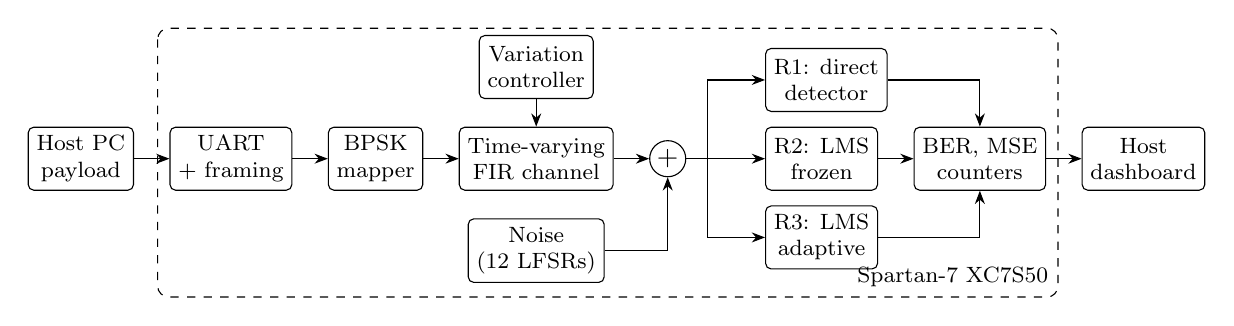
\begin{tikzpicture}[>=Stealth, node distance=0.35cm and 0.45cm,
  blk/.style={draw, rounded corners=2pt, align=center, font=\footnotesize, minimum height=0.8cm, inner sep=3pt}]
\node[blk] (host) {Host PC\\payload};
\node[blk, right=of host] (uart) {UART\\+ framing};
\node[blk, right=of uart] (map) {BPSK\\mapper};
\node[blk, right=of map] (ch) {Time-varying\\FIR channel};
\node[blk, above=of ch] (var) {Variation\\controller};
\node[blk, below=of ch] (noise) {Noise\\(12 LFSRs)};
\node[draw, circle, inner sep=1pt, right=of ch] (sum) {$+$};
\node[blk, right=1.0cm of sum, yshift=1.0cm] (r1) {R1: direct\\detector};
\node[blk, right=1.0cm of sum] (r2) {R2: LMS\\frozen};
\node[blk, right=1.0cm of sum, yshift=-1.0cm] (r3) {R3: LMS\\adaptive};
\node[blk, right=of r2] (cnt) {BER, MSE\\counters};
\node[blk, right=of cnt] (dash) {Host\\dashboard};
\draw[->] (host) -- (uart); \draw[->] (uart) -- (map); \draw[->] (map) -- (ch); \draw[->] (var) -- (ch);
\draw[->] (ch) -- (sum); \draw[->] (noise) -| (sum);
\draw[->] (sum) -- ++(0.5,0) |- (r1); \draw[->] (sum) -- (r2); \draw[->] (sum) -- ++(0.5,0) |- (r3);
\draw[->] (r1) -| (cnt); \draw[->] (r2) -- (cnt); \draw[->] (r3) -| (cnt); \draw[->] (cnt) -- (dash);
\draw[dashed, rounded corners] ($(uart.north west)+(-0.15,1.25)$) rectangle ($(cnt.south east)+(0.15,-1.35)$);
\node[font=\footnotesize, anchor=south east] at ($(cnt.south east)+(0.15,-1.35)$) {Spartan-7 XC7S50};
\end{tikzpicture}}
\caption{The experiment of the PPR. A variation controller drives the channel along a specified trajectory; one channel and one noise realisation feed three concurrent receivers, so differences between them are due to the adaptation rule alone. At mid-term the blocks from the BPSK mapper to the counters exist as Verilog (simulation only, \cref{sec:rtl}); UART, framing and host software do not.}
\label{fig:system}
\end{figure*}

\subsection{Receivers and adaptation source}
\label{sec:receivers}
\textbf{R1} detects $r[n]$ directly (the error floor). \textbf{R2} adapts during training and is frozen at $N_T$ (an equalizer matched to the channel as it was). \textbf{R3} keeps adapting. R1 and R2 are controls: R1 isolates the value of equalization, R2 the value of continued equalization. After training R3 needs an error reference. Three modes are distinguished and every result states which was used: \emph{decision-directed} ($\mathrm{sign}(y[n])$ replaces the reference \cite{sato1975,godard1980}, entered through a gate on a measured error level), \emph{pilot-assisted} (known symbols inserted periodically), and \emph{supervised} (the true symbol, available because the transmitter is internal to the experiment; used to isolate tracking from decision errors and never presented as a realisable receiver). \nb{The gate switches to decision-directed operation at the first $n\ge2000$ at which the running MSE (exponential average, time constant 1000 symbols) is below 0.1; otherwise the switch is forced at $N_T$ and flagged.}

\subsection{LMS, the tracking trade-off, delay and training}
\label{sec:lms}
With $\mathbf u[n]=[r[n],\ldots,r[n-L+1]]^T$, output $y[n]=\mathbf w^T[n]\mathbf u[n]$ and error $e[n]=x[n-\Delta]-y[n]$,
\begin{equation}
\mathbf w[n+1]=\mathbf w[n]+\mu\,e[n]\,\mathbf u[n],\qquad 0<\mu<\frac{2}{\mathrm{tr}(\mathbf R)},
\label{eq:lms}
\end{equation}
with $\mathbf R=E[\mathbf u\mathbf u^T]$ and $\mu$ a power of two in hardware. For a stationary channel the misadjustment $\mathcal M=\xi_{\rm ex}/J_{\min}$ grows roughly as $\mu\,\mathrm{tr}(\mathbf R)/2$ \cite{haykin2014}. For an optimum that moves as a random walk with increment covariance $\mathbf Q$, a lag term appears \cite{widrow1976,haykin2014,macchi1995}:
\begin{equation}
\mathcal M\approx\underbrace{\frac{\mu\,\mathrm{tr}(\mathbf R)}{2}}_{\text{gradient noise}}+\underbrace{\frac{\mathrm{tr}(\mathbf Q)}{2\mu J_{\min}}}_{\text{lag}},\qquad
\mu_{\rm opt}\approx\sqrt{\frac{\mathrm{tr}(\mathbf Q)}{J_{\min}\,\mathrm{tr}(\mathbf R)}}.
\label{eq:mis}
\end{equation}
The PPR's falsifiable prediction is an interior optimum step size that grows with the variation rate, as the square root of that rate.
\nb{Because $\mathrm{tr}(\mathbf Q)$ is the \emph{variance} of the increments, \eqref{eq:mis} makes $\mu_{\rm opt}$ proportional to the \emph{rms} increment (exponent 1 in the rms rate; the square root holds only for the variance). For a deterministic ramp of slope $v$ the lag term becomes $v^T\mathbf R^{-1}v/\mu^2$ and the first-order exponent is 2/3 \cite{bershad1989,vlaski2020}. (Eq.~\eqref{eq:mis} is Widrow \etal's Eqs.~81 and 86 \cite{widrow1976} rewritten for our step convention: their update uses $2\mu$, and their $n\sigma^2$ is our $\mathrm{tr}(\mathbf Q)$.) Our channel follows deterministic ramps, so both 1/2 (the PPR reference) and 2/3 are kept as reference slopes and the exponent is measured (\cref{sec:muopt}) and explained (\cref{sec:theory}). The gradient-noise term is corrected in \cref{sec:misadj}.}

The decision delay $\Delta$ is needed because the cascade $h*w$ can only approximate a delayed impulse; for a non-minimum-phase channel $\Delta=0$ asks a causal filter for an anti-causal inverse. $\Delta$ is chosen by sweeping $0\le\Delta\le L+M-2$, including the non-minimum-phase preset $h=[0.5,1.0]$ and its mirror $[1.0,0.5]$, and each receiver's bit offset is checked by cross-correlation. Training uses a maximal-length PRBS, $x^{15}+x^{14}+1$ (period 32767), to satisfy persistent excitation; $N_T=30000$ symbols for the continuous sweeps and 120000 for the abrupt transitions. \nb{A white symbol sequence gives white \emph{symbols}, but the equalizer sees them through the channel, so $\mathbf R\approx\mathbf H\mathbf H^T+\sigma^2\mathbf I$ rather than $\sigma^2\mathbf I$; the eigenvalue spread is set by the channel (up to 56 on the primary channel, \cref{sec:theory}). A PRBS-trained equalizer reaches MSE 0.0281 on random payload (oracle 0.0274); trained on $0,1,0,1,\ldots$ it reaches 0.9645 (\lvl{L1}).}

\subsection{Fixed-point model}
\label{sec:fixed}
Every width, rounding and saturation rule is explicit (\cref{tab:formats}); saturation is used rather than wraparound. Coefficients are held in an extended-precision accumulator whose top bits feed the multiplier, so the coefficient word length is two parameters: the accumulator width $B_{\rm acc}$, which decides whether small updates survive, and the multiplier width $B_{\rm mul}$, which sets the DSP cost \cite{constantinides2003,gitlin1982}. An update that falls below the accumulator's resolution is lost silently; on a moving channel the equalizer then stops while the channel does not. \nb{With rounding an update is lost when $|\mu e u|<\mathrm{LSB}/2$ \cite{shahdoosti2018}; this is a deadband, not an all-or-nothing stall, its effect depends on the rounding rule and on the statistics of $e$, and noise dithers updates across it. Because the trajectories are bounded, the resulting mismatch is bounded by the plateau of \cref{sec:metrics} rather than growing without limit.} The update loop is computed without pipelining ($D=0$), so the delayed-LMS bound \cite{long1989} is not needed. \nb{So that the RTL can match the software bit for bit, the channel and noise are formed in integers (tap $0.1\to6554/65536$, noise scaled by $\mathrm{round}(65536\sigma)$); on identical data this changes 3.4\,\% of received samples by one LSB and R3's MSE in the fifth digit.}

\begin{table}[t]
\centering\small
\caption{Bit-true fixed-point model (\lvl{L2}) and RTL formats. s$N$.$F$: signed, $N$ bits, $F$ fractional. Baseline $B_{\rm mul}=12$, $B_{\rm acc}=26$.}
\label{tab:formats}
\setlength{\tabcolsep}{3pt}
\begin{tabular}{@{}p{0.33\linewidth}p{0.27\linewidth}p{0.32\linewidth}@{}}
\toprule
Signal & Format & Rule\\
\midrule
$r$, delay line $u$ & s16.12 ($\pm8$) & round, saturate\\
coefficient accumulator & s$B_{\rm acc}$.($B_{\rm acc}-2$) & add update, saturate\\
multiplier coefficient & s$B_{\rm mul}$.($B_{\rm mul}-2$) & top bits, round, saturate\\
products, adder tree & $B_{\rm mul}+16$, $+20$ bits & exact\\
$y$, $e=d-y$ & s16.12 & round, saturate\\
update $\mu e u$, $\mu=2^{-p}$ & shift by $p$ & round or truncate\\
\bottomrule
\end{tabular}
\par\smallskip\footnotesize
\nb{Dynamic range checked: $|w|\le1.10$ in every LMS run (Wiener $|w|\le0.987$), $|r|\le2.73$, $|y|,|e|\le3.73$.}
\end{table}

\subsection{Metrics and statistics}
\label{sec:metrics}
Each path's BER is counted separately. The reacquisition time $N_{\rm rec}$ is the smallest $k$ such that the seed-averaged moving-average MSE (window 64) stays within a factor $1+\kappa$, $\kappa=0.25$, of the \emph{post}-transition steady level for all $n\ge N_C+k$ (the PPR's pre-transition reference is replaced because $h_A$ and $h_B$ have different attainable MSE). The PPR's tracking boundary $S^\star_{\rm BER}$ is the fastest rate at which R3 keeps its BER within a factor $f=2$ of its static-channel value, and $S_{\rm cross}$ the fastest rate at which R3 still outperforms both controls.

\nb{\emph{Statistics.} The static value is the measured static BER averaged over the channel states that the trajectory visits (the literal $c_{\rm lo}$ value is a sensitivity). A point passes or fails only if its 95\,\% paired seed-bootstrap interval lies entirely on one side of the threshold; otherwise it is inconclusive, and where the boundary point itself is inconclusive only a bracket is reported. The bootstrap was validated on 40 independent replicate experiments (coverage 92.5\,\% for nominal 95\,\%); errors come in bursts, so plain binomial intervals are kept only as sensitivities \cite{efron1993,wilson1927}. $S_{\rm cross}$ uses the same paired bootstrap on $\mathrm{BER}_{R3}-\min(\mathrm{BER}_{R1},\mathrm{BER}_{R2})$.}

\nb{\emph{MSE boundary.} A boundary in BER alone can be invisible while the eye is open, so an MSE boundary is added and never merged with it. The oracle $J_{\rm or}[n]$ is the minimum MSE of any $L$-tap equalizer that knows the channel taps active inside its window (checked against a 300\,000-trial brute-force computation to 0.3\,\%). With $\varepsilon=(J_{R3}-J_{\rm or})/J_{\rm or}$, $\varepsilon_{\rm static}(\mu)$ its static value and $\varepsilon_{\rm plateau}$ that of the best single fixed filter for the time-averaged channel, the tracking loss is
\begin{equation}
\rho=\frac{\varepsilon-\varepsilon_{\rm static}}{\varepsilon_{\rm plateau}-\varepsilon_{\rm static}},
\label{eq:rho}
\end{equation}
0 for no loss and about 1 for no better than a fixed filter. $S^\star_{\rm MSE}$ is the fastest $S$ that passes, i.e.\ whose 95\,\% seed-bootstrap upper bound of $\rho$ is below $\rho_{\rm th}=0.5$; it is a grid point, not the first failing rate and not an interpolated crossing (0.25 and 0.75 reported as bands); $\rho$ is undefined when $\varepsilon_{\rm static}\ge\varepsilon_{\rm plateau}$.}

\Cref{tab:params} lists the parameters. Rates and step sizes were fixed after simulation so that the grid brackets the boundary for every step size, as the PPR anticipated; the grid replaces the five provisional presets $S0$--$S4$. \nb{Pilot seeds 1000--1099 were used to choose these values, which were then frozen with a written checklist; all final results use the untouched seeds 2000--2099. A plain-numpy LMS reproduces the main loop to $10^{-15}$.}

\begin{table}[t]
\centering\small
\caption{Parameters of the final runs.}
\label{tab:params}
\setlength{\tabcolsep}{3pt}
\begin{tabular}{@{}p{0.3\linewidth}p{0.64\linewidth}@{}}
\toprule
Equalizer & $L=16$, $\Delta=2$\\
Step sizes & 14: $\mu=2^{-5},2^{-5.5},\ldots,2^{-11.5}$; the 7 powers of two are the FPGA set\\
Rates $S$ & 18: 5000, 2000, 1000, 500, 320, 224, 160, 112, 80, 56, 40, 28, 20, 14, 10, 5, 2, 1, and static\\
SNR & 16\,dB (MSE, primary), 14\,dB, 12\,dB (BER)\\
Seeds & 100 (2000--2099); 1500 for the 14\,dB BER study at $\mu\le2^{-7}$\\
Training & PRBS, $N_T=30000$ (continuous), 120000 (abrupt)\\
Evaluation & whole triangle periods, about 152000 symbols\\
Levels & \lvl{L1} float, \lvl{L2} bit-true, \lvl{L3} RTL simulation\\
\bottomrule
\end{tabular}
\end{table}

\section{Further Literature Review}
\label{sec:literature}
The PPR reviewed the origins of LMS and adaptive equalization, LMS tracking theory, decision-directed and normalised adaptation, and FPGA and fixed-point design. For the mid-term the literature was organised by development phase, so that each phase rests on its sources and each source is tied to the result it supports or contradicts (\cref{tab:litphase}). References already used in the PPR, and what they establish, are printed in black; \nb{sources added since the PPR, and every statement about our own results, are in blue. New sources were read at least at catalogue or abstract level; the depth is stated where it matters, and ``supports'' means that the source states the method or result we use, not that its derivations were re-checked.}

\noindent\textbf{P1 --- static LMS and validation.} The algorithm \cite{widrowhoff1960}, adaptive equalization \cite{lucky1965,qureshi1985}, the Wiener solution, misadjustment, eigenvalue spread and persistent excitation \cite{widrowstearns1985,haykin2014}, the BPSK error rate and the ISI model \cite{proakis2008}, and the equalizer delay set by the reference tap \cite{qureshi1985}. \nb{Mazo \cite{mazo1979} showed that the independence assumption on which LMS convergence theory rests is ``not even approximately true'' for a tapped-delay-line equalizer, although it often predicts well (abstract level). Our misadjustment finding (\cref{sec:misadj}) is a case where a consequence of that assumption --- a white residual error --- fails visibly, by a factor of 1.47. The PRBS and the noise LFSRs use maximal-length taps from Alfke \cite{alfke1996}.}

\noindent\textbf{P2 --- abrupt transitions.} Widrow \etal \cite{widrow1976} and Haykin \cite{haykin2014} give the learning-curve time constants $1/(\mu\lambda_i)$ and the role of the eigenvalue spread. \nb{Our recovery times follow $N_{\rm rec}\propto1/\mu$, and the slowest mode ($\lambda_{\min}\approx0.07$) explains why abrupt-transition runs need a longer training (\cref{sec:p2}).}

\noindent\textbf{P3--P4 --- continuous variation and the optimum step.} The gradient-noise/lag decomposition for a first-order Markov (random-walk) optimum \cite{widrow1976}, tracking in transmission \cite{macchi1995}, RLS tracking compared with LMS \cite{eleftheriou1986}, and statistical channel models \cite{jakes1974}. \nb{(The PPR described \cite{eleftheriou1986} as comparing ``across algorithm families''; it analyses RLS tracking and compares it with LMS.) For deterministic variation, Vlaski, Rizk and Sayed \cite{vlaski2020} show that a non-zero-mean drift turns the $1/\mu$ lag term into $1/\mu^2$ (read in full); Bershad and Macchi \cite{bershad1989} and an associated report \cite{dticada208618} treat LMS tracking of a chirp, with lag of order $v^{-2}$ (abstract level); Yousef and Sayed \cite{yousef2001} unify steady-state and tracking analysis; Bergmans \cite{bergmans1990} derives the lag error of LMS for a channel with band-limited gain variations and shows that the total error either rises monotonically with $\mu$ or has an interior minimum, depending on the size and bandwidth of the variation (read in full; replicated as R7). These sources give the 2/3 ramp alternative and the basis of the model of \cref{sec:theory}, which explains our measured exponent of 0.52--0.59. The statistics use the bootstrap \cite{efron1993} and the Wilson interval \cite{wilson1927}.}

\noindent\textbf{Adaptation source.} Sato \cite{sato1975} and Godard \cite{godard1980} established adaptation without a continuous training reference. \nb{Mazo \cite{mazo1980} analyses decision-directed start-up and notes that, because the symbol estimates can be wrong, convergence is not guaranteed (abstract level). Our measured divergence map (\cref{sec:dd}) quantifies this for our channel: divergence is set by $\mu$ and SNR, not by the variation rate.}

\noindent\textbf{P5 --- payloads.} \nb{The audio format (8\,kHz, 8 bits per sample) is the telephone-speech rate of ITU-T G.711 \cite{g711}; our samples are linear, not companded. The test image is a public-domain photograph distributed with scikit-image \cite{vanderwalt2014}.}

\noindent\textbf{P6 --- fixed point.} Delayed adaptation and its step bound \cite{long1989}, coefficient drift from bias in a digital update \cite{gitlin1982}, word-length selection \cite{constantinides2003}, FPGA LMS architectures \cite{hanson2016} and the DSP48E1 slice \cite{xilinxug479}. \nb{Ghanassi, Champagne and Kabal \cite{ghanassi2007} derive the steady-state error of fixed-point LMS for a stationary target, including a stall mode whose error grows as $1/\mu^2$; Shahdoosti \cite{shahdoosti2018} states the stall rule $|\mu e u|<\mathrm{LSB}/2$; Montenegro \etal \cite{montenegro2006} model stalling with Markov chains (record only); Khan and Gustafsson \cite{khan2023} study power-of-two step approximations. Our word-length study (\cref{sec:fxp}) is the tracking counterpart: the accumulator width, not the multiplier width, sets the boundary, and truncation needs about two more bits --- the drift that \cite{gitlin1982} anticipates. The sum of uniforms of the noise generator follows the Irwin--Hall distribution \cite{irwin1927,hall1927}, whose bounded tails we measured; Lee \etal \cite{lee2006} give the established higher-accuracy alternative. The FPGA LMS equalizers found were tested on static channels \cite{vargas2007} or used other algorithms \cite{kumari2021}; one thesis combines fixed-point LMS with time-varying channels on a DSP processor rather than an FPGA \cite{rierapalou2002}.}

\subsection*{Three key sources in detail}
\label{sec:keysources}
Three sources carry most of the weight of this report. For each, what it establishes and assumes is stated first, then \nb{what was reproduced and how our work goes beyond it. The type of agreement is named explicitly: \emph{exact numerical replication} (a published number is matched), \emph{reproduction of a theoretical trend} (a published functional form or scaling is matched), \emph{partial replication}, and \emph{independent validation} (our own model confirmed by another tool).}

\noindent\textbf{Widrow \etal \cite{widrow1976}} establish the learning behaviour of LMS for stationary and nonstationary inputs: the misadjustment due to gradient noise, and, for an optimum that drifts, the split of the excess error into gradient noise rising with $\mu$ and lag falling with $\mu$, with an optimum step between them, \eqref{eq:mis}. \nb{(Read in full.) The paper writes the update as $\mathbf w+2\mu e\mathbf u$, so its $\mu$ is half of ours; its results then read: misadjustment $\mu\,\mathrm{tr}(\mathbf R)$ (its Eq.~51, our $\mu\,\mathrm{tr}(\mathbf R)/2$), lag misadjustment $n\sigma^2/(4\xi_{\min}\mu)$ (Eq.~81), and $\mu^\star=[n\sigma^2/(4\xi_{\min}\mathrm{tr}\mathbf R)]^{1/2}$ (Eq.~86), which is exactly \eqref{eq:mis} with $\mathrm{tr}(\mathbf Q)=n\sigma^2$. Its assumptions are stated explicitly: input vectors uncorrelated over time and error independent of the input (Sec.~VIII); the formula valid for misadjustment up to about 25\,\%; a stationary input ($\mathbf R$ constant); each optimal weight an independent, slowly varying first-order Markov process, with the nonstationarity much slower than the adaptation (Sec.~XI); and white input, $\mathbf R=\mathbf I$, four weights and a 128-member ensemble in its tracking experiments. Two passages bear directly on our results. In its adaptive-predictor experiment the measured misadjustment exceeds the formula by 1.2--1.9 times (its Table~I; e.g.\ 3\,\% against 2.5\,\%), which the authors attribute to correlated input samples violating the uncorrelated-input assumption; our correction \eqref{eq:corrmis} quantifies that effect for an equalizer (\cref{sec:misadj}). Its footnote~4 notes that for a weight fluctuation with a different (uniform low-pass) spectrum the lag term changes its dependence on $\mu$, the optimum moves to where the gradient-noise loss is twice the lag loss, and the lag is ``quite sensitive to the spectral characteristics of the fluctuation'' --- the dependence we measure as a channel- and trajectory-dependent exponent (\cref{sec:theory}). Reproduced as theoretical trends: convergence to the Wiener filter, the misadjustment on a white input within 1--3\,\%, and the random-walk trade-off with $\mu_{\rm opt}$ within 1--9\,\% and exponent 1.000 (R3, R6). Beyond it: an ISI channel, where the white-residual assumption fails by a factor 1.47, and a deterministic, reversing ramp instead of a Markov drift.}

\noindent\nb{\textbf{Vlaski, Rizk and Sayed \cite{vlaski2020}} (read in full) analyse the steady-state tracking of stochastic-gradient learners, LMS included, when the optimum drifts. With a zero-mean (random-walk) drift the lag term scales as $1/\mu$; with a non-zero-mean, deterministic drift it scales as $1/\mu^2$; combined with the gradient-noise term, this gives an optimum-step exponent of 2/3 for a steady ramp. The analysis is first-order in a small step size and describes the steady state of a persistent drift. Reproduced as a theoretical trend: the ramp lag slope $-2.01$ and, with the exact gradient-noise term, the ramp optimum within 1--2.4\,\% (R6). Beyond it: our triangle reverses before the slowest eigen-direction of $\mathbf R$ reaches steady state, so the lag falls more slowly than $1/\mu^2$ and the measured exponent lies below 2/3 (0.52 primary, 0.58--0.59 control; \cref{sec:theory}).}

\noindent\nb{\textbf{Ghanassi, Champagne and Kabal \cite{ghanassi2007}} (read in full) derive the steady-state mean squared error of fixed-point LMS over the whole step-size range by splitting it into three modes: a stall mode, in which the quantised update rounds to zero and the error falls as $1/\mu^2$ (with two constants fitted to their simulations); a new intermediate mode; and the stochastic-gradient mode, in which quantisation acts as additive white noise. They assume a white stationary Gaussian input, a long filter, round-off quantisation of every product with no overflow, and a stationary system-identification target; their experiments use $N=100$, 16 bits and no additive noise. Reproduced: after correcting our rebuild to their two-quantiser update, our simulation matches their own simulation points within 0.72--1.19 for $\mu\le0.155$, except at the narrow error minimum with a wide accumulator (R5). Their formulas match their own points, and ours, only in parts (stall law 0.70--0.97, other modes within about a factor of two), so that difference belongs to the analysis, not to the replication. Beyond it: their analysis has no moving channel. Our word-length study measures how the same stalling mechanism moves the \emph{tracking} boundary of an equalizer on a time-varying ISI channel, and separates accumulator width from multiplier width and rounding from truncation (\cref{sec:fxp}).}

\noindent\nb{The remaining agreements are of the other two types: exact numerical replication for the BPSK BER and the stall onset at iteration 134 (R1, R4), and independent validation of our own Python LMS model, whose MSE and final coefficients a plain MATLAB implementation reproduces to every printed digit and MathWorks' equalizer within 1.2\,\% (\cref{sec:replication}).}

\noindent\textbf{Position.} The PPR observed that tracking analyses usually assume infinite precision and FPGA studies usually assume a static channel, and placed this project at their intersection. \nb{The further search did not find a study combining a bit-true fixed-point LMS equalizer, a swept deterministic variation rate, BER and MSE together, and a tracking limit. The search was short and not systematic, so this is stated only to the best of our knowledge; ``first'' or ``novel'' is not claimed.}

\noindent\nb{\textbf{Reference audit.} The audit checks that every claim the PPR makes from the literature rests on a source that exists and says what the PPR attributes to it. All 22 PPR references were checked against catalogue, publisher or author records (bibliographic details, and content at abstract level only): 10 were fully confirmed, 2 confirmed through a secondary citation, 7 partly confirmed and 3 not confirmed online; none was found wrong. Two papers were afterwards read in full, Widrow \etal \cite{widrow1976} (above) and Qureshi \cite{qureshi1985}, which is now confirmed (\emph{Proc.\ IEEE} 73(9), pp.~1349--1387). The audit led to two corrections: Qureshi does not single out non-minimum-phase channels, as the PPR stated, so that point now rests on our own delay sweep (\cref{sec:p1}); and the UG479 entry now carries its version and date. Nagumo--Noda \cite{nagumo1967} and the board manual \cite{realdigitalmanual} still need a library check.}

\begin{table*}[t]
\centering\footnotesize
\setlength{\tabcolsep}{3pt}
\caption{Literature by development phase. Black: references of the PPR and what they establish; \nb{blue: references added since the PPR, and our results.}}
\label{tab:litphase}
\begin{tabular}{@{}p{0.11\linewidth}>{\leavevmode}p{0.25\linewidth}>{\leavevmode}p{0.29\linewidth}>{\leavevmode\color{blue}}p{0.3\linewidth}@{}}
\toprule
Phase & References & What they establish & Our result (section)\\
\midrule
P1 & \cite{widrowhoff1960,lucky1965,qureshi1985,widrowstearns1985,haykin2014,proakis2008} \nb{\cite{mazo1979,alfke1996}} & LMS, Wiener solution, misadjustment, eigenvalue spread, BPSK BER, delay for non-minimum-phase channels; \nb{independence assumption; LFSR taps} & BER on theory; Wiener convergence; misadjustment 1.47$\times$ textbook (\cref{sec:p1})\\
P2 & \cite{widrow1976,haykin2014} & Time constants $1/(\mu\lambda_i)$ & $N_{\rm rec}\propto1/\mu$; slow-mode training (\cref{sec:p2})\\
P3--P4 & \cite{widrow1976,macchi1995,eleftheriou1986,jakes1974} \nb{\cite{vlaski2020,bershad1989,dticada208618,yousef2001,bergmans1990,efron1993,wilson1927}} & Lag vs gradient noise, optimum step; \nb{deterministic drift ($1/\mu^2$); bootstrap and binomial intervals} & Boundary $\approx0.11/\mu$; exponent 0.52--0.59, explained (\cref{sec:p3,sec:theory})\\
Adaptation & \cite{sato1975,godard1980} \nb{\cite{mazo1980}} & Adaptation without training; \nb{decision-directed convergence not guaranteed} & Divergence set by $\mu$ and SNR (\cref{sec:dd})\\
P5 & \nb{\cite{g711,vanderwalt2014}} & \nb{Telephone speech format; test image} & Audio and image results (\cref{sec:audio,sec:image})\\
P6 & \cite{long1989,gitlin1982,constantinides2003,hanson2016,xilinxug479} \nb{\cite{ghanassi2007,shahdoosti2018,montenegro2006,khan2023,irwin1927,hall1927,lee2006,vargas2007}} & Delayed LMS, coefficient drift, word length, FPGA LMS, DSP slice; \nb{stall mode and stall rule; sum-of-uniform noise; accurate hardware Gaussian noise} & Accumulator width sets the boundary; truncation needs $\approx$2 more bits; Irwin--Hall BER (\cref{sec:fxp,sec:replication})\\
\bottomrule
\end{tabular}
\end{table*}

\section{Replication of Published Results}
\label{sec:replication}
Each published result was rebuilt from its description, run independently and compared with what the source states; no source code was available. \nb{A result counts as \emph{reproduced} only when a stated number or functional form is matched within the stated tolerance, and nothing was tuned to improve agreement. \Cref{fig:scorecard} compares our values with the published or theoretical ones and \cref{tab:replication} classifies each replication; \cref{fig:repl} shows the comparisons themselves.}

\begin{figure*}[t]
\centering
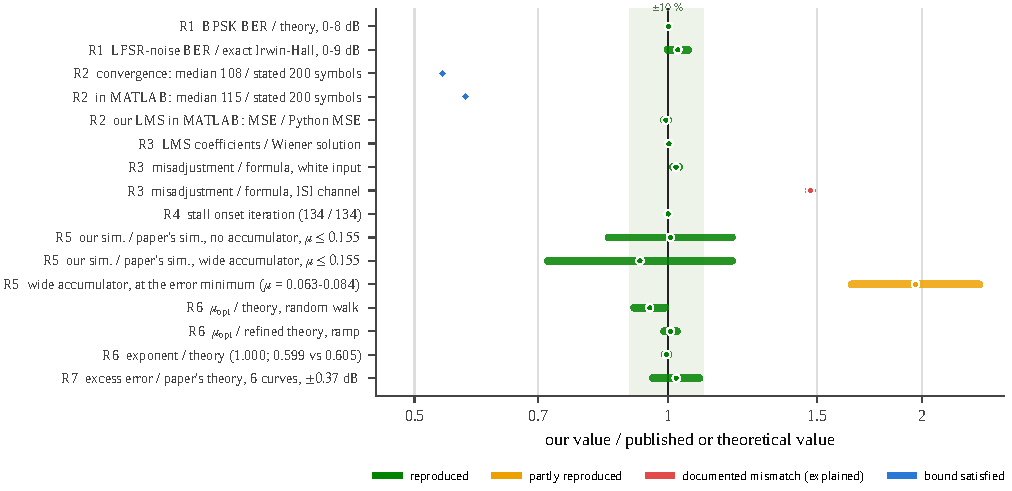
\includegraphics[width=0.8\linewidth]{figs/scorecard.pdf}
\caption{\nb{Replication scorecard: our value divided by the published or theoretical value (bars: range over the stated conditions; shaded: $\pm10$\,\%). Most reproduced results lie inside $\pm10$\,\%; the R5 bands are wider because they include about $\pm5$\,\% digitising error of the paper's points. The R3 ISI point is the documented misadjustment mismatch, explained in \cref{sec:misadj}; R2 is an upper bound (``less than 200 symbols''), satisfied with margin by our model and by MATLAB; MathWorks' LMS run on our own samples agrees with our model within 1.2\,\%.}}
\label{fig:scorecard}
\end{figure*}

\textbf{R1 --- BPSK in AWGN.} The flat-channel error rate is $Q(\sqrt{2E_b/N_0})$ \cite{proakis2008}. \nb{Simulated BER / theory is 1.000--1.002 for 0--8\,dB ($2\times10^7$ symbols) and 0.95/0.92 at 9/10\,dB with 639/71 errors, statistically consistent. For the 12-uniform hardware noise, the exact Irwin--Hall BER \cite{irwin1927,hall1927} is matched to 0.998--1.056 (\cref{fig:repl}a).}

\textbf{R2 --- MathWorks ``Equalize a BPSK signal''} \cite{mathworks}: an 8-tap LMS equalizer, step 0.1, channel $[0.02+0.5j,\ 0.05]$, 30\,dB, 200 training symbols; the page states that the equalizer ``converges in less than 200 bits''. \nb{Our re-implementation converges at a median of 108 symbols (5--95\,\%: 97--123), 1000/1000 runs within 200, with no post-training errors (\cref{fig:repl}b). Assumed, because the page does not state them: the complex LMS convention and the initial weights; both initialisations give the same result. This channel is nearly ISI-free after derotation, so the example tests convergence, not ISI removal. The original example was also run in MATLAB R2025b with MathWorks's own equalizer (\texttt{comm.LinearEqualizer}, 1000 runs): median 115 symbols (5--95\,\%: 103--133), 1000/1000 runs under 200 symbols and 1000/1000 without post-training errors. The two medians differ by about 7 symbols (6\,\%), plausibly through MATLAB's initial weights and alignment convention, which the page does not state; the published claim is confirmed by both.}

\nb{\emph{MATLAB cross-check of our own LMS model.} On our received samples (primary channel at $c=40$ and $c=116$, 14\,dB, 16 taps, $\mu=2^{-8}$), MathWorks' LMS equalizer gives a steady-state MSE of 0.022449 and 0.055030 against our 0.022469 and 0.055690 (ratios 0.999 and 0.988, at its best reference tap), and the same LMS equations written as a plain MATLAB loop reproduce our MSE and final coefficients to every printed digit (ratio 1.00000). The Python model is therefore confirmed by an independent tool (\lvl{L1}).}

\textbf{R3 --- stationary LMS theory.} LMS converges to the Wiener filter and its misadjustment is about $\mu\,\mathrm{tr}(\mathbf R)/2$ \cite{widrow1976,haykin2014}. \nb{Convergence to the Wiener filter (coefficients within 0.17--0.18\,\%) and the misadjustment formula on a white-input control (within 1--3\,\%) are reproduced. On the ISI channel the measured excess is 1.47--1.48 times the formula; this documented mismatch is explained in \cref{sec:misadj}.}

\nb{\textbf{R4 --- stall onset} \cite{shahdoosti2018}: AR(10) signal with the paper's initial values, $\mu=0.01$, 12 fractional bits, rounding. The paper reports that stalling begins at iteration 134, with the threshold $e_T=\mathrm{LSB}/(2\mu u)=0.0244$ for $u=0.5$. Our first iteration with all updates rounded to zero is \textbf{134} (\cref{fig:repl}c). The paper does not state how the desired signal is formed; one-step prediction was assumed. With truncation instead of rounding the onset is 129--130, so the agreement depends on the rounding rule that the paper states.}

\nb{\textbf{R5 --- fixed-point steady-state error} \cite{ghanassi2007} (read in full): $N=100$ taps, 16 bits, white Gaussian input of variance 0.1, $\|\mathbf w_o\|^2=0.4$, no noise, with and without a wide accumulator. An earlier rebuild, made from a partly unreadable copy, rounded the update $\mu e\mathbf u$ once; the full text shows two quantisers, first $Q[\mu e]$ and then $Q[Q[\mu e]\,u]$ (its Eqs.~5b, 17). The rebuild was corrected and nothing else changed, then run at the paper's own step sizes and compared with the paper's \emph{simulation} points, digitised from its Figs.~2 and 3 (reading error about $\pm5$\,\%). For $\mu\le0.155$ our steady-state error is 0.85--1.19 times the paper's at all 18 points without accumulator, and 0.72--1.19 times at 15 of 18 points with it (\cref{fig:repl}d). The exceptions are the narrow error minimum of the accumulator variant ($\mu=0.063$--0.084, 1.65--2.34 times), where the error is only a few times the quantisation floor, and the last points before the stability limit $\mu<0.2$ ($\mu\ge0.169$), where the error rises steeply and a small difference in $\mu$ changes it by orders of magnitude. The paper's \emph{formulas}, by contrast, match both its own points and ours only in parts: the stall law within 0.70--0.97, the intermediate formula within about 1.3 without accumulator, the stochastic-gradient formula within 0.54--0.86. That gap lies between the paper's analysis and its own experiment, not in our rebuild. One modelling choice was made after seeing a result: building the reference from the unquantised input adds a $10^{-5}$ floor from rare input saturation, absent from the paper's results, so the quantised reference was used. \emph{Reproduced (the paper's simulation), with the two stated exceptions.}}

\textbf{R6 --- the tracking trade-off \eqref{eq:mis}} \cite{widrow1976,haykin2014,macchi1995}\nb{, with the deterministic-drift form of \cite{vlaski2020,bershad1989}: system identification with 8 taps, white input, and a random-walk or deterministic-ramp optimum (\cref{fig:repl}e). The lag slopes $-1$ (random walk) and $-2.01$ (ramp) and the gradient-noise slope $+1$ are reproduced; $\mu_{\rm opt}$ agrees with \eqref{eq:mis} within 1--9\,\% and the measured random-walk exponent is 1.000. For the ramp the exponent is 0.60 instead of the first-order 2/3, because the optimum moves to large $\mu$ where the first-order gradient-noise term is too small; with the exact white-input term the theory gives 0.605 and the optimum agrees within 1--2.4\,\%. This is the same finite-step effect found on our own channel (\cref{sec:theory}).}

\nb{\textbf{R7 --- LMS tracking of gain variations} \cite{bergmans1990} (read in full): LMS identification of a 5-tap channel $f_0=1$, $f_2=-1$ whose output is scaled by $1+g_k$, with $g_k$ a first-order autoregressive (low-pass) gain of bandwidth $\beta$; binary input, Gaussian noise, $c_0=f$, 16384 samples per $\mu$. The paper derives the excess error as gradient noise (its Eq.~10) plus a lag error (its Eq.~27), predicts from its Eq.~32 whether the total error rises monotonically with $\mu$ or has a minimum, and reports simulation within about $\pm0.2$\,dB of theory in its Figs.~2--4. All six curves of those figures were rebuilt (20 runs per point). Our simulation lies within $-0.18$ to $+0.14$\,dB of the theory on four curves and within $+0.23$ and $+0.37$\,dB on the two with $\beta=0.1$ at 25\,dB and at 5\,\% gain variation, in the middle range of $\mu$ (\cref{fig:repl}f). The monotone/minimum classification of Eq.~32 is confirmed on all six curves; the minimum is 2.4\,dB deep at 5\,\% (theory 2.6\,dB), 1.35\,dB at 25\,dB (theory 1.5\,dB) and only 0.1\,dB at 20\,dB, 2\,\%, where its position is not resolvable. The residual excess disappears (all curves within $\pm0.18$\,dB) when the lag error is also counted as a driver of gradient noise ($N_0\to N_0+\varepsilon_l$ in Eq.~10); this is a diagnostic, not a change to the verdict, and it is the same mechanism as our misadjustment correction (\cref{sec:misadj}): an error that the filter cannot remove adds to the gradient noise. \emph{Reproduced}, with a slightly larger deviation than the stated $\pm0.2$\,dB on two curves.}


\begin{table}[t]
\centering\small
\caption{\nb{Replications by type. Levels: R1--R3, R6 and R7 \lvl{L1}; R4 and R5 are small stand-alone fixed-point models, not the project's \lvl{L2}.}}
\label{tab:replication}
\color{blue}
\setlength{\tabcolsep}{3pt}
\begin{tabular}{@{}lp{0.47\linewidth}p{0.36\linewidth}@{}}
\toprule
& Quantity & Type of replication\\
\midrule
R1 & BPSK BER; exact BER of the LFSR noise & exact (numerical)\\
R2 & MathWorks example, convergence $<200$ & qualitative (bound); confirmed in MATLAB\\
R3 & Wiener convergence; misadjustment & exact on white input; mismatch on ISI, explained\\
R4 & stall onset at iteration 134 & exact\\
R5 & fixed-point steady-state error & paper's simulation reproduced, except at the accumulator minimum and near instability; its formulas only partly\\
R6 & lag/noise trade-off, $\mu_{\rm opt}$ scaling & exact (functional form)\\
R7 & excess error with gain variations; monotone or minimum & functional form, within $\pm0.37$\,dB; classification exact\\
\bottomrule
\end{tabular}
\end{table}

\begin{figure*}[t]
\centering
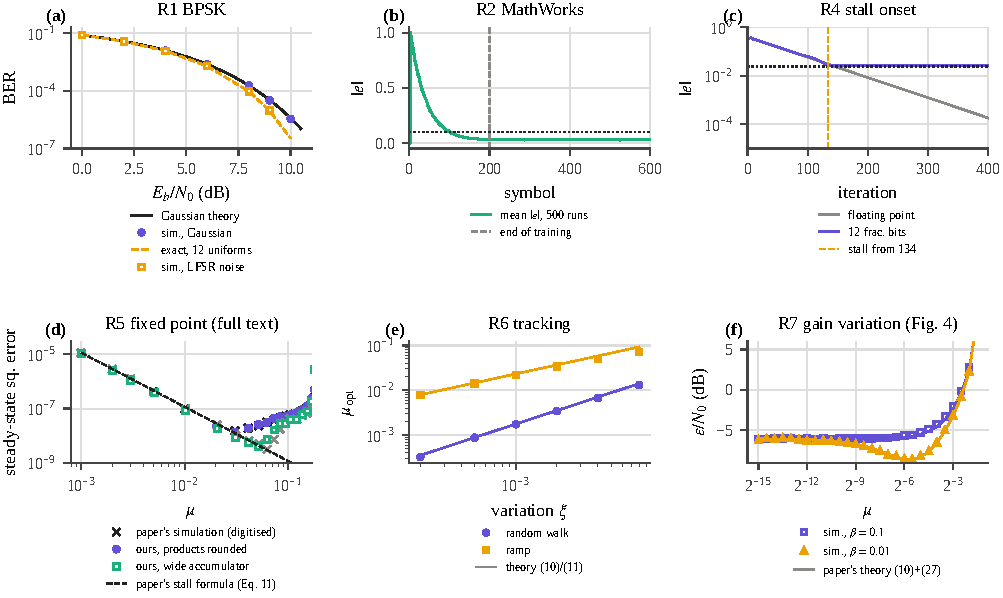
\includegraphics[width=\linewidth]{figs/replication.pdf}
\caption{\nb{Replications (\lvl{L1}; R4, R5 stand-alone fixed-point models). (a)~R1: BPSK BER against Gaussian theory, and the LFSR (12-uniform) noise against its exact Irwin--Hall BER. (b)~R2: mean error magnitude of the MathWorks 8-tap equalizer over 500 runs; it falls below 0.1 at about 100 symbols, inside the 200-symbol training. (c)~R4: error magnitude of fixed-point LMS; every update rounds to zero from iteration 134, as published, while floating point keeps converging. (d)~R5, rerun after reading the full text: our steady-state error and the paper's own simulation points at the same step sizes, with its stall formula \cite{ghanassi2007}. (e)~R6: optimum step against the variation for a random-walk and a ramp optimum, with theory; the ramp departs at large $\mu$ (finite-step effect). (f)~R7: excess error against step size for the case of Fig.~4 of \cite{bergmans1990} (20\,dB, 5\,\% rms gain variation), with the paper's theory; the narrow-band gain ($\beta=0.01$) gives a minimum, the wide-band one ($\beta=0.1$) a monotone rise.}}
\label{fig:repl}
\end{figure*}

\section{Simulation Results: P1--P4}
\label{sec:results14}
All results in this section are \lvl{L1} (floating point, Gaussian noise), supervised unless stated, with the parameters of \cref{tab:params}.

\subsection{P1: validation of the apparatus}
\label{sec:p1}
Before any tracking result, the PPR required the flat-channel BER against theory, the static-ISI error floor and its removal, convergence to the Wiener filter, the choice of $\Delta$ and the check of the training sequence. \nb{On a flat channel the BER at 12 SNR points ($2\times10^6$ bits each) lies on $Q(\sqrt{2E_b/N_0})$, with 11 of 12 points inside their 95\,\% interval and all 12 inside 99\,\% (\cref{fig:p1}a); this checks noise scaling, threshold, SNR definition and bit counting together. On static ISI channels R1 has an error floor (14--20\,\% at $a=0.91$ at every SNR) that matches its exact analytic BER, and R2/R3 remove it (no errors in $10^6$ bits at 16\,dB; \cref{fig:p1}b). LMS converges to the Wiener filter (average coefficients within 0.17--0.18\,\%), the oracle agrees with a brute-force computation to 0.32\,\%, and the bit-alignment, PRBS and noise tests pass. One test fails: the textbook misadjustment.}

\begin{figure*}[t]
\centering
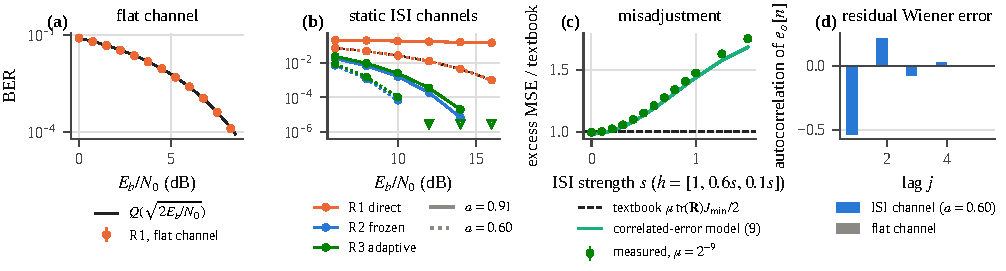
\includegraphics[width=\linewidth]{figs/p1.pdf}
\caption{P1 validation (\lvl{L1}). (a)~Flat-channel BER of the direct detector against BPSK theory. (b)~Static ISI channels ($a=0.91$ solid, $0.60$ dotted): R1 against its exact BER (black), and R2, R3. \nb{Triangles: no errors observed (plotted at the 95\,\% upper bound). (c)~Measured excess MSE divided by the textbook misadjustment, against ISI strength, with the correlated-error model \eqref{eq:corrmis}; the textbook value holds only on a flat channel. (d)~Autocorrelation of the Wiener filter's residual error: strongly negative at lag 1 on the ISI channel, zero on a flat channel.}}
\label{fig:p1}
\end{figure*}

\subsubsection*{\nb{Correction of the misadjustment formula}}
\label{sec:misadj}
\nb{On the control channel ($a=0.60$, 14\,dB) the measured excess MSE is \textbf{1.47--1.48 times} $\mu\,\mathrm{tr}(\mathbf R)J_{\min}/2$ (16 independent seeds of $10^6$ symbols, 95\,\% intervals $\pm0.003$), while on a white-input flat channel the same measurement matches the formula within 1--3\,\% and halves when $\mu$ halves. The formula assumes that the error $e_o$ left by the optimum filter is white and independent of the input. On an ISI channel that residual is mostly leftover interference, so neighbouring errors are strongly correlated (lag-1 correlation $-0.53$, \cref{fig:p1}d). Keeping that correlation in the first-order analysis gives
\begin{equation}
\begin{aligned}
\xi_{\rm ex}&\approx\tfrac{\mu}{2}\Big(C(0)-2\textstyle\sum_{j\ge1}C(j)\Big),\\
C(j)&=E\big[e_o[n]\,e_o[n-j]\,\mathbf u^T[n]\mathbf u[n-j]\big],
\end{aligned}
\label{eq:corrmis}
\end{equation}
where $C(j)$ is computed exactly from the channel, without simulation. Here $C(0)=0.606$ equals $J_{\min}\mathrm{tr}(\mathbf R)$ within 0.6\,\%, but $\sum_{j\ge1}C(j)=-0.144$, so \eqref{eq:corrmis} predicts $(0.606+0.288)/0.609=1.468$ times the textbook value, against 1.468--1.480 measured. Shuffling the data in time, which removes the correlation, restores the textbook value (ratio 0.99--1.00). Widrow \etal already observed measured misadjustment 1.2--1.9 times above the formula in their adaptive predictor and attributed it to correlated input samples \cite[Table~I]{widrow1976}; \eqref{eq:corrmis} turns that observation into a prediction. Over ISI strength the ratio rises from 1.00 (flat) to 1.75 ($a=0.90$), and \eqref{eq:corrmis} follows it within 1.5--4\,\% (\cref{fig:p1}c). The textbook form is therefore an incorrect use of an approximation here, not a simulation error, and \eqref{eq:corrmis} is used for all predictions in this report.}

\noindent\textbf{Decision delay and alignment.} The PPR expected a clear MSE minimum against $\Delta$ and a large difference between a non-minimum-phase channel and its mirror. \nb{For $h=[0.5,1.0]$ the Wiener MSE at $\Delta=0$ is 0.756 (LMS 0.797) against 0.025 at the best delay ($\Delta\approx6$--11, flat); for the mirror $[1.0,0.5]$ it is 0.026 at $\Delta=0$ (\cref{fig:delay}). Identical magnitude responses give a factor of 30 in MSE, and LMS follows the Wiener curve at every $\Delta$, about 5\,\% above it. On the project channels the best $\Delta$ is 3--7 (primary) and 5--7 (control), but the minimum is so flat that the fixed $\Delta=2$ costs at most 1.3\,\% MSE, and only 0.07--0.27\,\% on the moving channel; $\Delta$ therefore need not follow the channel. The cross-correlation peak equals the predicted offset for every receiver (lag 0 for R1, 2 for R2 and R3); a wrong offset gives BER 0.499--0.503.}

\begin{figure}[t]
\centering
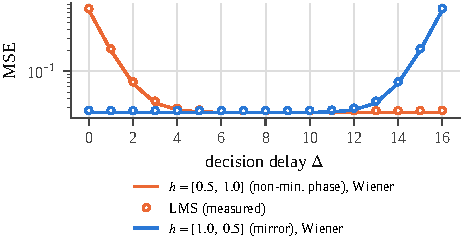
\includegraphics[width=\linewidth]{figs/delay.pdf}
\caption{Decision-delay sweep for the non-minimum-phase preset $h=[0.5,1.0]$ and its mirror, 14\,dB (\lvl{L1}): Wiener MSE (lines) and measured LMS (circles). \nb{The two channels have the same magnitude response; the non-minimum-phase one needs $\Delta\ge5$.}}
\label{fig:delay}
\end{figure}

\subsection{P2: abrupt transitions and reacquisition}
\label{sec:p2}
The MSE around each step (\cref{fig:p2}) and $N_{\rm rec}$ against $\mu$ (\cref{fig:nrec}) were planned to show reacquisition. R3 reacquires while R2 stays at the mismatched level. \nb{The recovery time is inversely proportional to the step size: the log--log slopes of $N_{\rm rec}$ against $\mu$ are $-1.06/-1.00/-0.98$ at 16\,dB and $-1.03/-1.02/-0.97$ at 14\,dB for the three steps, against $-1.07\ldots-1.00$ from the noise-free mean-weight model $E[\mathbf w]=\mathbf w_B+(\mathbf I-\mu\mathbf R_B)^k(\mathbf w_A-\mathbf w_B)$. On the harsh step the measured value lies above the model (e.g.\ 3386 against 3067 symbols at $\mu=2^{-8}$), the expected one-sided bias of a last-crossing statistic, and individual values there are uncertain by about $\pm20$\,\%. R2 after the step matches its analytic frozen-filter MSE (e.g.\ 0.395 against 0.393).}

\nb{\emph{Training length.} With $N_T=60000$, R2 after the ``down'' step was 0.7--3.0\,\% \emph{better} than an ideally trained filter. The mean-weight model predicted why: the slowest direction of $\mathbf R$ ($\lambda_{\min}\approx0.07$ at $c=116$) still held about 1\,\% weight error after 60000 symbols, invisible on the training channel. With $N_T=120000$ the offset fell to $-0.6\ldots+0.05$\,\% (at $\mu=2^{-10}$: $-2.31\to+0.05$\,\%, model $-2.10\to\approx0$). Small residual offsets (up to $+1.7$\,\% at 14\,dB, $\mu=2^{-7}$, falling with $\mu$) remain \emph{unexplained} and are reported as measured; the $N_T=60000$ results are preserved.}

\begin{figure*}[t]
\centering
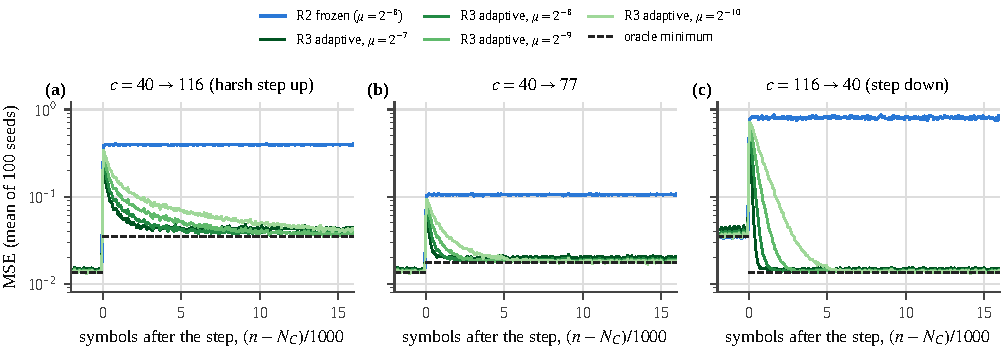
\includegraphics[width=\linewidth]{figs/p2.pdf}
\caption{Abrupt transitions at $N_C$, primary channel, 16\,dB, 100 seeds, $N_T=120000$ (\lvl{L1}): MSE against time for R2 and for R3 at four step sizes; dashed: oracle minimum before and after the step. \nb{R3 reacquires, faster for larger $\mu$; R2 stays at the mismatched level.}}
\label{fig:p2}
\end{figure*}

\begin{figure}[t]
\centering
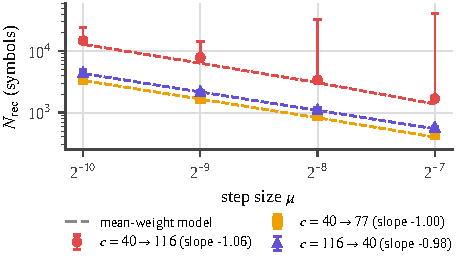
\includegraphics[width=\linewidth]{figs/p2nrec.pdf}
\caption{Reacquisition time $N_{\rm rec}$ against $\mu$ for the three steps, 16\,dB, 100 seeds (\lvl{L1}): measured (95\,\% seed bootstrap) and mean-weight model (dashed). \nb{All three follow $N_{\rm rec}\propto1/\mu$; the wide intervals on the harsh step come from the noisy last-crossing statistic.}}
\label{fig:nrec}
\end{figure}

\subsection{P3: tracking against the variation rate}
\label{sec:p3}
The PPR's principal result is the BER of R1, R2 and R3 against the variation rate on identical data (\cref{fig:ber}). R1 and R2 are flat, because they never adapt and every evaluation window covers whole up-and-down periods, so they see the same mix of channel states at every speed; only R3's error depends on speed, which is what the experiment isolates. R3 holds its static BER at slow variation and rises towards a ceiling at fast variation.

\begin{figure*}[t]
\centering
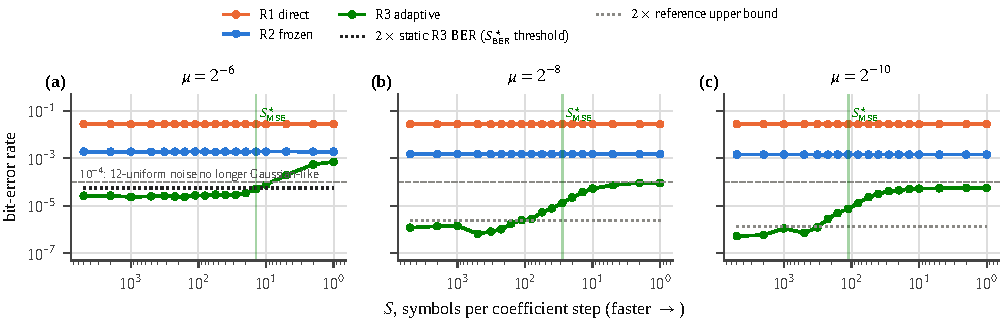
\includegraphics[width=\linewidth]{figs/ber_vs_S.pdf}
\caption{BER against variation rate for R1, R2 and R3, primary channel, 14\,dB, 100 seeds (\lvl{L1}, Gaussian noise). Dotted: the $S^\star_{\rm BER}$ threshold, $2\times$ the static R3 BER. Dashed: $10^{-4}$, below which the planned 12-uniform hardware noise no longer approximates Gaussian BER (\cref{sec:channel}); these \lvl{L1} curves use Gaussian noise. \nb{Green line: $S^\star_{\rm MSE}$. R3 loses BER at slower rates as $\mu$ falls; it stays below R2 at every rate for these $\mu$.}}
\label{fig:ber}
\end{figure*}

\nb{\emph{MSE boundary.} The tracking loss $\rho$ rises from 0 to about 1 as $S$ falls (\cref{fig:rho}). $S^\star_{\rm MSE}$ is bracketed inside the grid in all 68 cases where $\rho$ is defined, and never shows a pass after a non-pass. For $\mu\le2^{-7.5}$ it is the same on both channels at 14 and 16\,dB (within one grid step at 12\,dB) and doubles each time $\mu$ halves: $S^\star_{\rm MSE}\cdot\mu=0.109$--0.110 (\cref{fig:bound}a, \cref{tab:sstar}). At larger $\mu$ the static misadjustment uses up part of the room below the plateau and the boundary flattens; at $\mu=2^{-5}$, 12--14\,dB, $\rho$ is undefined. \Cref{sec:theory} derives this law.}

\nb{\emph{What the boundary means.} $S$ is the number of symbols between successive one-step changes of the channel coefficient, so a smaller $S$ is a faster-changing channel. $S^\star_{\rm MSE}$ is the fastest rate on the tested grid at which R3's tracking loss is still statistically below half of the way to a fixed filter (\cref{sec:metrics}). The law $S^\star_{\rm MSE}\approx0.11/\mu$ says that, within the tested regime, \emph{halving the step size requires doubling the number of symbols between channel changes} --- the channel must change half as often --- to keep the same tracking accuracy: a smaller step averages out more noise but adapts proportionally more slowly. The law is measured for these two channels, $L=16$, 12--16\,dB and $\mu\le2^{-7.5}$; it is not a universal property of adaptive equalizers or of physical channels, and at larger $\mu$ the static misadjustment bends it (\cref{fig:bound}a).}

\begin{figure*}[t]
\centering
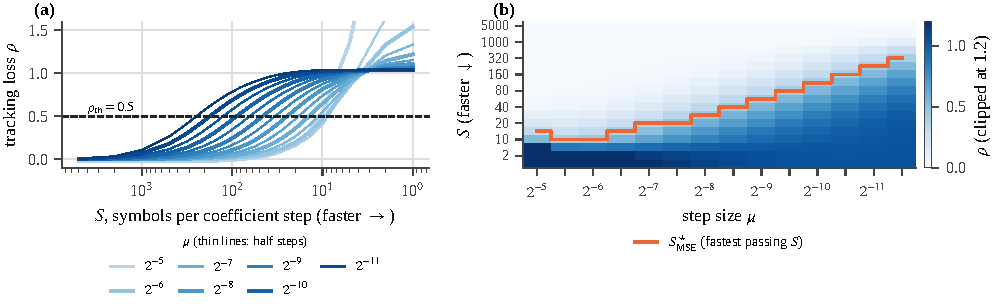
\includegraphics[width=\linewidth]{figs/rho.pdf}
\caption{\nb{Tracking loss $\rho$ \eqref{eq:rho}, primary channel, 16\,dB, all 14 step sizes, 100 seeds (\lvl{L1}). (a)~$\rho$ against $S$; $S^\star_{\rm MSE}$ is the fastest rate at which the curve is still statistically below 0.5 (not the interpolated crossing). (b)~The same data as a map over $(\mu,S)$; the orange staircase is $S^\star_{\rm MSE}$ (the fastest passing rate), which moves one rate step slower each time $\mu$ halves.}}
\label{fig:rho}
\end{figure*}

\nb{\emph{BER boundary} ($f=2$). $S^\star_{\rm BER}$ lies 1--3 grid steps \emph{slower} than $S^\star_{\rm MSE}$ (\cref{fig:bound}b; e.g.\ $\mu=2^{-8}$: $S^\star_{\rm MSE}=28$, $S^\star_{\rm BER}=56$ at 12\,dB and 112 at 14\,dB). It is stricter because a BER threshold of twice the static value is a small \emph{absolute} change once the static BER is small: a modest rise in MSE moves a few more received samples across the decision threshold and doubles a $10^{-6}$ BER long before the MSE loses half of its tracking margin. For the same reason it is stricter at higher SNR, where the static reference BER is smaller. At 16\,dB the reference is measurable only for $\mu\ge2^{-5.5}$; elsewhere passes are reference-limited. Where the boundary point itself is inconclusive, only the bracket is given.}

\noindent\textbf{BER and MSE compared.} The PPR posed the research question in terms of BER, and BER remains the receiver's figure of merit. \nb{At 14--16\,dB, however, the static R3 BER is $10^{-7}$--$10^{-6}$, and so a BER boundary needs $10^{8}$ or more bits per point and is often reference-limited (\cref{tab:sstar}). MSE is measured on every symbol and is resolved with 100 seeds at every grid point. MSE is therefore used as the statistically resolved reference, and the following check, which uses only the existing \lvl{L1} runs, tests whether it ranks the operating points as BER does. \Cref{fig:bermse} plots R3's BER against its MSE $J$ at every $(\mu,S)$ grid point with at least 20 errors. If the error at the slicer were Gaussian, BPSK would give}
\begin{equation}
\nb{\mathrm{BER}_{\rm G}=Q\!\left(1/\sqrt{J}\right).}
\label{eq:bergauss}
\end{equation}
\nb{Two results follow. (i)~\emph{For a fixed step size, BER and MSE move together}: as the channel speeds up, both rise. The rank correlation over $S$ is at least 0.84 for every $\mu$ at 12 and 14\,dB, with a median of 0.90--1.00; at 16\,dB the minimum is 0.62 for $\mu\ge2^{-6}$ and 0.85 for $\mu\le2^{-7}$, where fewer errors are counted. Both metrics therefore order the variation rates in the same way, and an MSE boundary marks a real BER degradation. (ii)~\emph{The mapping from MSE to BER is not unique.} At equal MSE a larger step size gives a higher BER (\cref{fig:bermse}), and \eqref{eq:bergauss} underestimates the measured BER. The measured value is 0.5--128 times $\mathrm{BER}_{\rm G}$ for $\mu\le2^{-7}$ and 2--2000 times for $\mu\ge2^{-6}$ (12--16\,dB). The slicer error is a mix of residual ISI and noise, and $J$ is an average over channel states whose BER contributions are very unequal, so the error is not Gaussian. MSE is therefore a precise reference for \emph{where} tracking is lost, but it cannot replace BER as a measure of \emph{how many} bits are lost. Both metrics are kept and reported separately, and the stricter BER boundary (above) is consistent with this comparison.}

\begin{figure}[t]
\centering
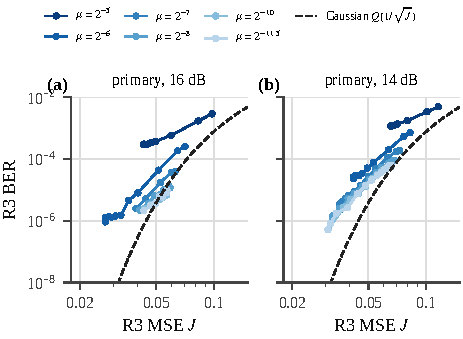
\includegraphics[width=\linewidth]{figs/bermse.pdf}
\caption{\nb{R3 BER against R3 MSE on the primary channel (\lvl{L1}, 100 seeds; points with at least 20 errors). Each line is one step size, traced over the variation rates (slow at the left, fast at the right). Dashed: the Gaussian prediction \eqref{eq:bergauss}. For a fixed $\mu$, BER rises with MSE; across step sizes, equal MSE does not mean equal BER.}}
\label{fig:bermse}
\end{figure}

\begin{figure*}[t]
\centering
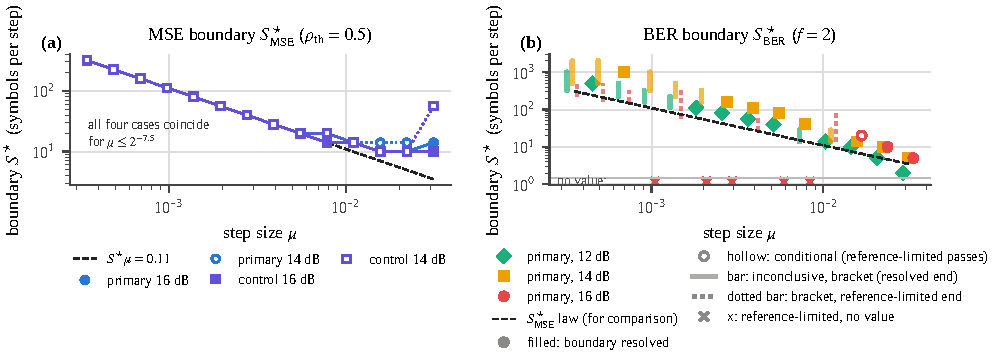
\includegraphics[width=\linewidth]{figs/boundaries.pdf}
\caption{\nb{Tracking boundaries against step size, primary and control channels (\lvl{L1}, supervised, 100 seeds; 1500 at 14\,dB for $\mu\le2^{-7}$). $S$ is the number of symbols between channel changes, so a larger $S^\star$ means the receiver already loses tracking at a slower channel. (a)~$S^\star_{\rm MSE}$, the fastest grid rate at which the tracking loss is statistically below 0.5: for $\mu\le2^{-7.5}$ all four cases coincide on $S^\star\mu\approx0.11$, i.e.\ halving $\mu$ doubles the required $S$. (b)~$S^\star_{\rm BER}$ ($f=2$) on the primary channel at 12, 14 and 16\,dB, with every outcome shown: filled marker, boundary resolved; hollow marker, conditional (passes limited by the measurable reference); bar, boundary point statistically inconclusive, so only the bracket between the last pass and the first failure is known (dotted when the pass end is reference-limited); $\times$, no value can be claimed because the reference BER is too small to measure. The BER boundary lies at slower variation than the MSE boundary and moves further as the SNR rises.}}
\label{fig:bound}
\end{figure*}

\begin{table*}[t]
\centering\small
\caption{\nb{Tracking boundaries (\lvl{L1}, 100 seeds). $S^\star_{\rm MSE}$ ($\rho_{\rm th}=0.5$) and $S^\star_{\rm BER}$ ($f=2$, primary channel). u: $\rho$ undefined. n.d.\ [a, b]: boundary point inconclusive, transition between $S=a$ and $S=b$. R: resolved; C: conditional (reference-limited passes). Half-power step sizes follow the same pattern (full tables in the code package).}}
\label{tab:sstar}
\color{blue}
\setlength{\tabcolsep}{4pt}
\begin{tabular}{@{}l|ccccc|ccc@{}}
\toprule
& \multicolumn{5}{c|}{$S^\star_{\rm MSE}$} & \multicolumn{3}{c}{$S^\star_{\rm BER}$, primary}\\
$\mu$ & prim.\ 16 & prim.\ 14 & prim.\ 12 & ctrl.\ 16 & ctrl.\ 14 & 12\,dB & 14\,dB & 16\,dB\\
\midrule
$2^{-5}$ & 14 & u & u & 10 & 56 & 2 (R) & 5 (R) & 5 (R)\\
$2^{-6}$ & 10 & 14 & 14 & 10 & 10 & 10 (R) & 14 (R) & 20 (C)\\
$2^{-7}$ & 20 & 20 & 20 & 14 & 20 & n.d.\ [28, 14] & 40 (R) & ref.-limited\\
$2^{-8}$ & 28 & 28 & 28 & 28 & 28 & 56 (R) & 112 (R) & n.d.\ [56, 28]\\
$2^{-9}$ & 56 & 56 & 56 & 56 & 56 & 112 (R) & n.d.\ [320, 160] & ref.-limited\\
$2^{-10}$ & 112 & 112 & 112 & 112 & 112 & n.d.\ [320, 160] & n.d.\ [1000, 320] & ref.-limited\\
$2^{-11}$ & 224 & 224 & 160 & 224 & 224 & 500 (R) & n.d.\ [2000, 500] & n.d.\ [500, 160]\\
\bottomrule
\end{tabular}
\end{table*}

\noindent\textbf{Usefulness against the controls ($S_{\rm cross}$).} The PPR asked where the adaptive receiver ceases to outperform its controls, and expected that R2 might match or beat R3 under very slow variation. \nb{On the primary channel R3's BER advantage over both R1 and R2 is demonstrated at \emph{every} $S$ down to $S=1$, for all $\mu\le2^{-6}$ at 12, 14 and 16\,dB. A loss of advantage is confirmed only for $\mu=2^{-5}$ at $S\le2$, where R3's gradient noise is largest. One point, $\mu=2^{-5.5}$ at 16\,dB and $S=1$, is inconclusive (BER $8.30\times10^{-4}$ for R3 against $8.01\times10^{-4}$ for R2); no significant advantage is demonstrated there and no equivalence is claimed. On the control channel at 16\,dB most points are inconclusive because all three receivers make almost no errors. R3 therefore loses tracking \emph{accuracy} ($\rho>0.5$) long before it stops being \emph{useful}: losing half of the tracking margin still leaves a lagging filter that is much closer to the moving optimum than a filter frozen at the training channel (R2) or no filter at all (R1), whose errors are set by the full channel mismatch (\cref{fig:traj}). R2 never matched R3 on the primary channel, because even a slow triangle sweeps the whole channel range, away from R2's training state.}

\subsection{P4: the optimum step size}
\label{sec:muopt}
The step-size study tests the prediction \eqref{eq:mis} of an interior optimum that grows with the variation rate. \nb{For every $S$ an interior optimum $\mu_{\rm opt}$ exists and grows with $1/S$ (\cref{fig:muopt}a). The fitted exponent ${\rm d}\log_2\mu_{\rm opt}/{\rm d}\log_2(1/S)$ is 0.519, 0.525 and 0.511 on the primary channel (16/14/12\,dB) and 0.593 and 0.575 on the control channel (16/14\,dB). The seed-only 95\,\% interval is $\pm0.0005$; the real uncertainty is the systematic band over seven pre-declared fit variants, about $\pm0.03$ (e.g.\ 0.487--0.543 at 16\,dB; error bars in \cref{fig:muopt}b). The exponent is channel-dependent and lies between the random-walk 1/2 and the steady-ramp 2/3, and its local slope changes along $S$. The PPR's square-root prediction happens to describe the primary channel; \cref{sec:theory} shows why, and that this is not evidence of random-walk behaviour.}

\begin{figure*}[t]
\centering
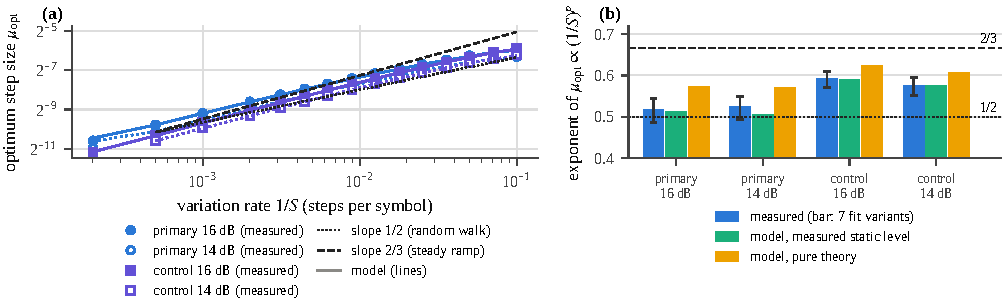
\includegraphics[width=\linewidth]{figs/muopt.pdf}
\caption{Optimum step size against the variation rate (\lvl{L1}, supervised, 100 seeds). (a)~Measured $\mu_{\rm opt}$ (markers) for both channels at 14 and 16\,dB, \nb{the theory model of \cref{sec:theory} (lines)}, and reference slopes 1/2 and 2/3 (their vertical position is arbitrary; only the slope matters). \nb{(b)~Fitted exponent $p$: measured (error bar: range over seven pre-declared fit variants, the dominant uncertainty), model with the measured static level, and pure first-order theory. The primary-channel exponent (0.52) is consistent with 1/2 within its uncertainty; the control-channel exponent (0.58--0.59) lies between 1/2 and 2/3. The model with the measured static level reproduces both within 0.02.}}
\label{fig:muopt}
\end{figure*}

\subsection{Coefficient trajectories}
\label{sec:traj}
The PPR planned to overlay the LMS coefficients on the known optimum trajectory (\cref{fig:traj}). \nb{At $S=1000$ the filter follows (relative rms coefficient error 0.022) with a lag of about 950--1300 symbols; at $S=1000$ the lag scales as $1/\mu$ (168, 400, 1072, 1952, 3440 symbols for $\mu=2^{-6}\ldots2^{-10}$, log--log slope $-1.10$). At $S=56$, twice the boundary, the coefficient swing shrinks to 64--73\,\% of the optimum's (error 0.16); at $S=14$, half the boundary, to 28--39\,\% (error 0.26): the filter traces a delayed, shrunken copy of the optimum. This is what the boundary means physically.}

\begin{figure*}[t]
\centering
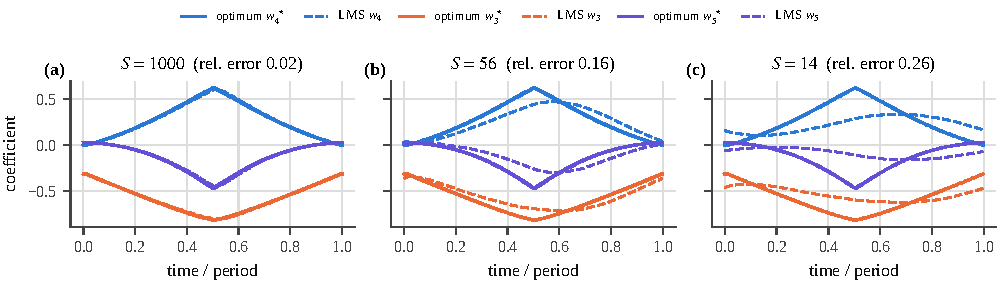
\includegraphics[width=\linewidth]{figs/traj.pdf}
\caption{The three most-moving coefficients over one period: exact moving optimum (solid) and LMS (dashed, mean of 20 seeds), $\mu=2^{-8}$, 16\,dB (\lvl{L1}). \nb{(a)~$S=1000$: LMS follows. (b)~$S=56$ and (c)~$S=14$ ($S^\star_{\rm MSE}=28$): LMS lags and its swing shrinks.}}
\label{fig:traj}
\end{figure*}

\subsection{Triangle against sinusoid}
\label{sec:trisin}
The PPR chose a triangular trajectory because it needs no sine hardware, and committed to checking in floating point that the triangle and a sinusoid give comparable tracking at matched average rates of change. \nb{A sinusoid with the same extremes, start point and period has the same average rate $|{\rm d}a/{\rm d}n|=2^{-7}/S$ but a peak rate $\pi/2$ times larger. Over $S=1000\ldots5$, three step sizes and 20 seeds (\cref{fig:trisin}), the two give the same kind of tracking curve, but at matched average rate the sinusoid is harder: R3's excess MSE is 5--36\,\% higher and, where tracking dominates, the sinusoid behaves like a triangle running 1.2--1.6 times faster. Matched at \emph{peak} rate, the two agree within $-24\ldots+34$\,\% over most of the range. Part of the difference is not tracking: the sinusoid dwells longer near the harsh end, which also raises R1's BER ($2.7\to3.9\times10^{-2}$). The two families are therefore comparable when matched at peak rate; at matched average rate the triangle is not a worst case.}

\begin{figure}[t]
\centering
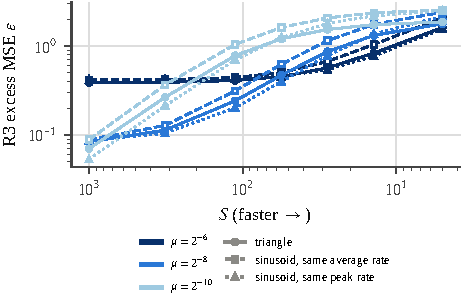
\includegraphics[width=\linewidth]{figs/trisin.pdf}
\caption{Triangle against sinusoid, primary channel, 16\,dB, 20 seeds (\lvl{L1}): R3's oracle-normalised excess MSE $\varepsilon$ against $S$. \nb{At matched average rate the sinusoid is harder; matched at peak rate the curves nearly coincide.}}
\label{fig:trisin}
\end{figure}

\subsection{Decision-directed and pilot-assisted operation}
\label{sec:dd}
The PPR required the decision-directed divergence threshold to be measured and reported, and the supervised results to be checked against realisable modes. \nb{At 14\,dB, for $\mu=2^{-6},2^{-8},2^{-10}$ and all $S$ from 1000 down to 1 (20 seeds), decision-directed, pilot-assisted (one pilot every 10 or 50 symbols) and supervised R3 give the same BER and MSE within statistical noise; R3's own decision error rate there is at most $7.3\times10^{-4}$. \emph{The supervised tracking results above therefore also describe a realisable decision-directed receiver on this channel at 14\,dB for $\mu\le2^{-6}$.} Divergence is set by the step size and the SNR, not by the variation rate (\cref{fig:dd}; $S=28$ and $S=1000$ behave alike): $\mu=2^{-5}$ loses lock at every SNR, $\mu=2^{-6}$ at $\le10$\,dB (1/20 runs at 10\,dB, 8/20 at 8\,dB, 20/20 at 6\,dB), and $\mu\le2^{-7}$ is safe down to 6\,dB. Too short a training also breaks it: forcing the switch after 25--50 training symbols loses lock in 20/20 runs, after 100 symbols in 9--19/20, after $\ge200$ symbols in none. Abrupt jumps $40\leftrightarrow116$ at 6--14\,dB never broke decision-directed adaptation at $\mu=2^{-8}$.}

\begin{figure}[t]
\centering
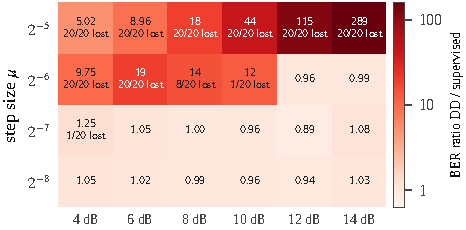
\includegraphics[width=\linewidth]{figs/dd.pdf}
\caption{Decision-directed operation, primary channel, $S=28$, 20 seeds (\lvl{L1}). \nb{Cell: BER of decision-directed R3 divided by supervised R3 on identical data; ``lost'': runs that lost lock. Values near 1 mean decision-directed operation is as good as supervised; the boundary runs diagonally in $(\mu,\mathrm{SNR})$.}}
\label{fig:dd}
\end{figure}

\section{Applications and Fixed-Point Results: P5--P6}
\label{sec:results56}

\subsection{P5: recorded audio}
\label{sec:audio}
A short mono recording is quantised, sent through the link and reconstructed once per receiver, so that a tracking failure becomes audible; the recording is replayable, which keeps the comparison fair. This is channel equalization, not acoustic noise cancellation. \nb{The payload is a 19.9\,s voice recording of a team member at 8\,kHz, mono, 8-bit (1\,271\,128 bits), run at 14\,dB with $\mu=2^{-8}$ and one seed (\lvl{L1}, \emph{supervised}). On the moving channel R1 loses about 2\,\% of the bits and R2 about 0.1\,\%, in long blocks wherever the channel coefficient is large; R3 keeps the BER at $10^{-6}$--$10^{-5}$ (\cref{fig:audio}). R3's waveform SNR against the 8\,kHz original falls from 30.6\,dB (static) to 29.6, 21.7 and 20.0\,dB at $S=1000$, 28 and 1, with 1, 3, 16 and 58 bit errors. An independent re-implementation from the specification reproduced the error counts within random variation.} One listener (a team member) heard R3 clearly better than R2, and R2 than R1; this is a subjective note, and the measurements are BER and waveform SNR. Because the adaptation is supervised, this demonstrates tracking, not a realisable audio receiver. \nb{Decision-directed operation matched supervised operation at this SNR and step size in the communication tests of \cref{sec:dd}; it was not run on the audio payload itself.}

\begin{figure*}[t]
\centering
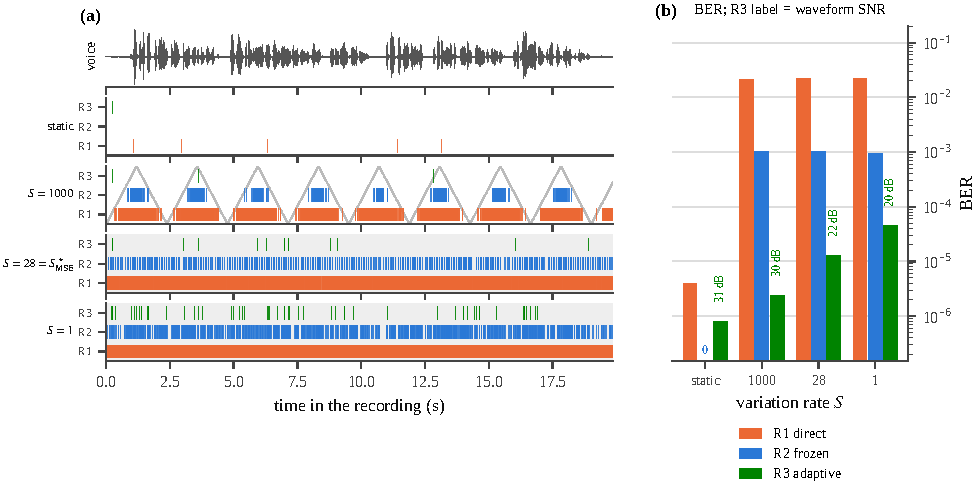
\includegraphics[width=\linewidth]{figs/audio.pdf}
\caption{Recorded voice through the time-varying primary channel, 14\,dB, $\mu=2^{-8}$, one seed (\lvl{L1}, supervised). (a)~The waveform and the position of every bit error of R1, R2 and R3 for a static channel and $S=1000$, 28 and 1 (grey: channel coefficient $a[n]$; shaded: too fast to draw). \nb{(b)~BER per receiver and scenario; R3 is labelled with its waveform SNR. At $S=1000$, R1 and R2 fail in blocks wherever $a[n]$ is large, while R3's errors stay isolated; R3 degrades gracefully from 31 to 20\,dB as the channel speeds up.}}
\label{fig:audio}
\end{figure*}

\subsection{Image payload}
\label{sec:image}
The PPR predicted that, because position in the image corresponds to elapsed time, R2 would degrade progressively down the image while R3 does not, until at fast enough variation R3 also fails. \nb{The $128\times72\times8$-bit image (a public-domain photograph shipped with scikit-image \cite{vanderwalt2014}; 5 seeds) shows both behaviours. At 14\,dB the differences are small (R2 53--90 wrong pixels, R3 0--12), so lower SNRs were run. At $S=1000$ the channel ramps once across the image and R2 degrades down the image: its BER per band of 8 rows rises from 0 to $1.4\times10^{-2}$ at 12\,dB and from $2\times10^{-5}$ to $2.5\times10^{-2}$ at 10\,dB, while R3 stays below $2\times10^{-4}$ and $1.4\times10^{-3}$ (\cref{fig:imgstats}a). R3 also fails, in both senses used here: at 10\,dB and $\mu=2^{-8}$ its BER rises from $1.4\times10^{-5}$ (static) to $1.5\times10^{-3}$ at $S=5$ and 1 (about 100 wrong pixels, 100 times its static value), and with $\mu=2^{-5}$ at $S=1$ it becomes \emph{worse than R2} (1027 against 649 wrong pixels; mean absolute pixel error 4.65 against 2.42), matching the confirmed loss of advantage in \cref{sec:p3} (\cref{fig:imggrid,fig:imgstats}b). Errors are spread evenly over the eight bit planes.} The PPR's earlier $128\times72$ result (4,911 and 380 errors) \nb{cannot be reproduced, because its channel, noise level and step size were not recorded, and is superseded by these results.}

\begin{figure}[t]
\centering
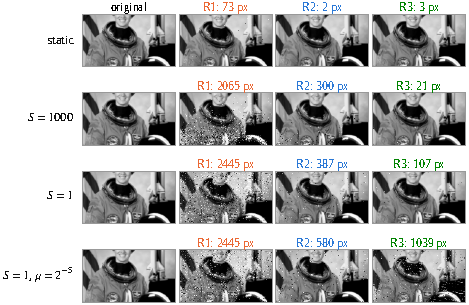
\includegraphics[width=\linewidth]{figs/image_grid.pdf}
\caption{Image payload at 10\,dB, one seed (\lvl{L1}, supervised; $\mu=2^{-8}$ unless stated). Columns: original, R1, R2, R3, with wrong-pixel counts. \nb{R2 degrades towards the bottom as the channel ramps; at $S=1$ with $\mu=2^{-5}$ R3 is worse than R2.}}
\label{fig:imggrid}
\end{figure}

\begin{figure*}[t]
\centering
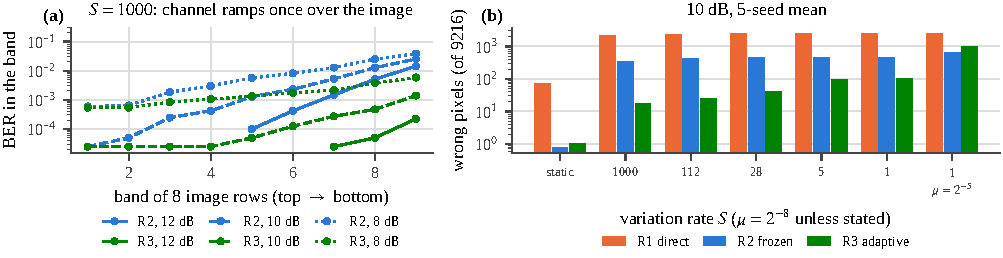
\includegraphics[width=\linewidth]{figs/image_stats.pdf}
\caption{\nb{Image payload statistics (\lvl{L1}, supervised, 5 seeds). (a)~BER per band of 8 image rows at $S=1000$, where the channel ramps once over the image: R2's BER rises down the image by two to three orders of magnitude, R3's much less. (b)~Wrong pixels at 10\,dB against the variation rate: R3 stays far below R2 until $S\approx5$, and with $\mu=2^{-5}$ at $S=1$ it is worse than R2.}}
\label{fig:imgstats}
\end{figure*}

\subsection{P6: word length against tracking (\lvl{L2})}
\label{sec:fxp}
The PPR's precision study asks how much coefficient precision is needed to sustain tracking at a given rate, with coefficient-update underflow as the expected mechanism. The bit-true model of \cref{tab:formats} uses the same LMS equations as \lvl{L1}. \nb{Four levels of agreement are kept apart: numerical equality of values, agreement of bit decisions, agreement of BER, and preservation of the tracking boundary. \emph{Equivalence:} with very wide words ($B_{\rm mul}=24$, $B_{\rm acc}=48$) the bit decisions equal \lvl{L1} (0 differences in $3.8\times10^6$); the values are not identical (MSE within $2.3\times10^{-7}$, coefficients within $4.6\times10^{-5}$) because signals are still quantised to s16.12. \emph{Static cost:} an 8-bit multiplier costs 2--9\,\% MSE, 12 and 16 bits $\le0.2$\,\%. \emph{Stalls:} the measured fraction of stalled updates matches a prediction from \lvl{L1} data (e.g.\ 0.466 against 0.489); with rounding, even 47\,\% stalled updates cost only $+0.33$\,\% MSE because the noise dithers the updates, whereas truncation biases the filter ($+31$\,\% at $\mu=2^{-11}$, 16-bit accumulator). $N_{\rm rec}$ is unchanged by word length.}

\nb{\emph{Tracking boundary against word length} (\cref{fig:fxp}; 112 configurations, all seven FPGA step sizes, 20 seeds, 16\,dB). (1)~The \emph{accumulator} width sets the boundary and the \emph{multiplier} width does not: with $B_{\rm acc}=26$, $B_{\rm mul}=8$, 12 and 16 give the same $S^\star_{\rm MSE}$ at every $\mu$, and the 8-bit multiplier costs only static accuracy (static excess 8.2/22.4\,\% against 4.5/11.5\,\% at the two channel ends, $\mu=2^{-8}$). (2)~With rounding, $B_{\rm acc}\ge16$ never moves the boundary; 14 bits move it only at $\mu=2^{-11}$, 12 bits from $2^{-8}$, 10 bits from $2^{-6}$. Smaller steps need more accumulator bits --- the underflow mechanism. (3)~Truncation needs about two more bits than rounding. \emph{Design consequence:} with round-to-nearest updates and $B_{\rm mul}=12$, a 16-bit accumulator gives the same $S^\star_{\rm MSE}$ grid point as the 26-bit baseline at all seven power-of-two step sizes, and the 26-bit row equals the \lvl{L1} boundary on the same rate grid. This is preservation of the \emph{MSE tracking boundary} (16\,dB, primary channel, 20 seeds); it does not mean that values, coefficients or BER are identical, and the BER boundary was not measured at reduced width. Using 16 rather than 26 accumulator bits is therefore a \emph{software-supported design recommendation}, not a measured saving in resources or timing.} This answers the PPR's hypothesis: \nb{underflow can restrict tracking, but only below these widths or with truncation.}

\noindent\textbf{Engineering significance.} The research question is how fast a \emph{fixed-point} LMS equalizer can track; the word-length study answers the fixed-point part. \nb{(i)~\emph{Why the accumulator matters.} Tracking is carried by many small coefficient updates $\mu e u$; each update must survive being added to the stored coefficient, so the accumulator's resolution decides whether the filter keeps moving. Smaller $\mu$ makes the updates smaller, which is why the required accumulator width grows as $\mu$ falls (\cref{fig:fxp}a). (ii)~\emph{Rounding against truncation.} Rounding loses updates below half an LSB symmetrically, and the channel noise dithers them, so the loss averages out; truncation always rounds the same way, which adds a systematic drift to every coefficient and costs about two more bits for the same boundary. (iii)~\emph{Diminishing return from the multiplier.} The multiplier width only sets how precisely the stored coefficient is used in the filter output; beyond 12 bits the output error it adds is far below the channel noise (static MSE cost $\le0.2$\,\%), and it never touches the update path, so it does not move the boundary. (iv)~\emph{What it suggests for the FPGA.} The extended-precision accumulator of the PPR can be narrower than the 26-bit baseline, with round-to-nearest, while the multiplier stays at 12 bits, within one DSP48E1 input. (v)~\emph{What it does not show.} These are \lvl{L2} results for one channel and SNR; RTL verification at the chosen widths, synthesis, timing analysis and board measurements (P8--P10) are still needed before any resource or speed claim.}

\begin{figure*}[t]
\centering
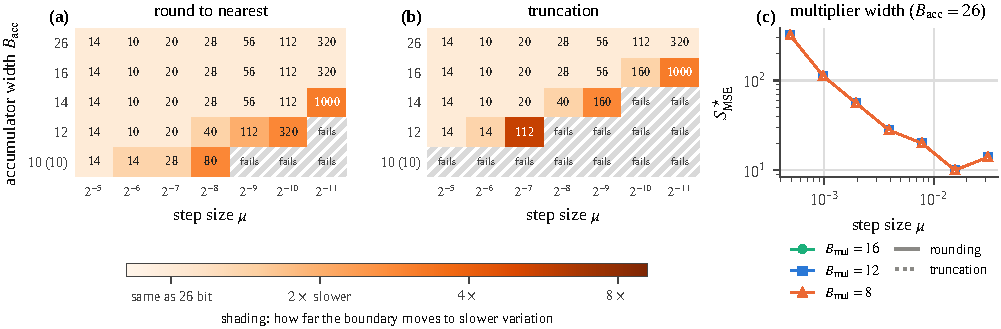
\includegraphics[width=\linewidth]{figs/fxp.pdf}
\caption{Tracking boundary $S^\star_{\rm MSE}$ against coefficient word length, primary channel, 16\,dB, 20 seeds, supervised (\lvl{L2}, bit-true; rate grid without $S=224$). \nb{(a),~(b)~Accumulator width $B_{\rm acc}$ with round-to-nearest and with truncated updates; multiplier width 12 bits (10 where shown in brackets). Each cell gives $S^\star_{\rm MSE}$; the shading shows how far the boundary moves to slower variation relative to the 26-bit row; ``fails'': the filter fails even on a static channel. (c)~Multiplier width 8, 12 and 16 bits with a 26-bit accumulator: all six curves coincide, so the multiplier does not limit tracking. With rounding, $B_{\rm acc}\ge16$ gives the same MSE boundary as 26 bits at every FPGA step size; values, coefficients and BER are not claimed identical.}}
\label{fig:fxp}
\end{figure*}

\subsection{First RTL (P7--P8, \lvl{L3}, ahead of schedule)}
\label{sec:rtl}
P7--P8 were planned for the final report and have started. Verilog exists for the 12-LFSR noise generator, the PRBS, the variation controller, the channel-plus-noise front end, R1, R2 and R3 ($L=16$; parameterised $B_{\rm mul}$, $B_{\rm acc}$, $\mu$ and rounding) and the error and MSE counters, in one chain. \nb{In iverilog simulation, the noise stream (20\,000 samples) and the full chain (7 configurations $\times$ 6000 symbols, including truncation, heavy stalling, saturation, a static and a fast ($S=1$) channel) are identical to the \lvl{L2} model in every per-symbol signal and every counter; Verilator lint reports no errors.} The code is behavioural: widths must be trimmed and the multipliers mapped to DSP48E1 slices before synthesis. \emph{No synthesis, timing, resource or board result exists.}

\section{\nb{Interpretation: a Theory Model of the Boundary and the Optimum Step}}
\label{sec:theory}
\begin{newtext}
\Cref{sec:p3,sec:muopt} report measurements. This section derives them from first-order LMS theory applied to the actual channel, with no fitted constant and no LMS simulation, so that every headline number has two independent sources.

\subsection{Model}
Following the two terms of \eqref{eq:mis}, R3's excess MSE is split into lag and gradient noise, each computed for the real trajectory instead of a random walk.
\emph{Lag.} Under the usual independence assumption the mean coefficient vector obeys the deterministic recursion
\begin{equation}
\bar{\mathbf w}[n+1]=\bar{\mathbf w}[n]+\mu\big(\mathbf p[n]-\mathbf R[n]\,\bar{\mathbf w}[n]\big),
\label{eq:meanw}
\end{equation}
started from the Wiener filter of the training channel, where $\mathbf R[n]$ and $\mathbf p[n]$ are the exact moving-window statistics of the time-varying channel (the same as the oracle's). The lag excess $\varepsilon_{\rm lag}(\mu,S)$ is $J_n(\bar{\mathbf w}[n])-J_{\rm or}[n]$, averaged over the evaluation window and divided by the mean oracle MSE.
\emph{Gradient noise.} The correlated-error result \eqref{eq:corrmis}, computed for every channel state and averaged over the time the triangle spends there: $\varepsilon_{\rm gn}(\mu)\propto\mu$.
\emph{Predictions.} $\varepsilon=\varepsilon_{\rm lag}+\varepsilon_{\rm gn}$; $\rho=\varepsilon_{\rm lag}/(\varepsilon_{\rm plateau}-\varepsilon_{\rm gn})$; $S^\star_{\rm MSE}$ as the fastest grid rate with $\rho<0.5$ (the measurement rule, without the bootstrap), and the continuous crossing $x^\star$ where $\rho=0.5$ exactly; $\mu_{\rm opt}(S)=\arg\min_\mu\varepsilon$. A \emph{semi-empirical} variant uses the measured static excess in place of $\varepsilon_{\rm gn}$, to test the lag part alone.

\subsection{Agreement with the measurements}
\emph{Boundary:} for $\mu\le2^{-7.5}$ the pure-theory model gives the measured $S^\star_{\rm MSE}$, at the resolution of the rate grid, \textbf{in all 40 cases} (2 channels $\times$ 14 and 16\,dB $\times$ 10 step sizes; \cref{fig:model}a). For $\mu\ge2^{-7}$ it is mostly one grid step too fast, and at $\mu=2^{-5}$ up to three steps, because the first-order gradient noise is too small there (by a factor 0.48--0.65); the semi-empirical variant removes most of that error. \emph{Lag:} predicted/measured lag excess has median 0.98 (10--90\,\%: 0.84--1.00) over 143--177 points per case. \emph{Exponent} (\cref{fig:muopt}b): the semi-empirical model gives 0.512, 0.505, 0.591 and 0.575 against the measured 0.519, 0.525, 0.593 and 0.575 (primary 16/14\,dB, control 16/14\,dB), within 0.02 and with the right channel dependence; pure theory gives 0.573, 0.570, 0.623 and 0.607, 0.03--0.05 too high for the same large-$\mu$ reason --- the finite-step effect also found in replication R6.

\begin{figure*}[t]
\centering
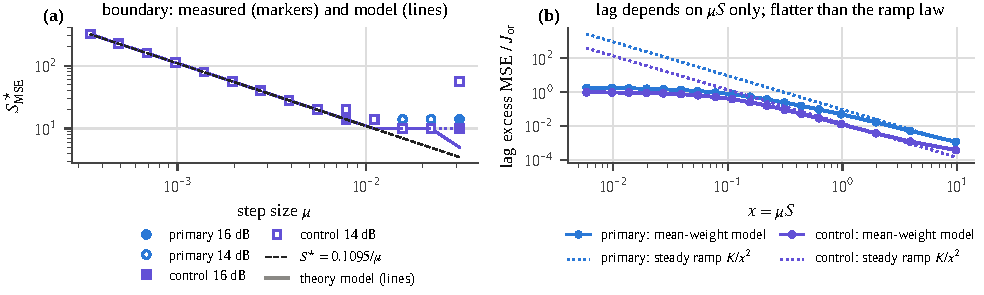
\includegraphics[width=\linewidth]{figs/model.pdf}
\caption{Theory model against measurement (\lvl{L1}; the model runs no LMS simulation). (a)~$S^\star_{\rm MSE}$ against $\mu$, measured (markers) and pure-theory model (lines), with $S^\star=0.1095/\mu$; for $\mu\le2^{-7.5}$ the model gives the measured grid point in all 40 cases. (b)~Lag excess against $x=\mu S$ from the mean-weight model at $\mu=2^{-9}$, with the steady-ramp law $K/x^2$ (dotted): the lag depends on $\mu S$ only, and on the primary channel it falls much more slowly than the ramp law, which is why the exponent is below 2/3.}
\label{fig:model}
\end{figure*}

\subsection{Why $S^\star_{\rm MSE}\propto1/\mu$}
In \eqref{eq:meanw} the channel moves one counter step every $S$ symbols while the filter moves at rate $\mu$. Rescaling time by $S$ shows that the lag depends on $\mu$ and $S$ almost only through
\begin{equation}
x=\mu S,
\label{eq:x}
\end{equation}
the adaptation progress made per channel step (checked: $\varepsilon_{\rm lag}$ at fixed $x$ changes by at most 2\,\% between $\mu=2^{-8}$ and $2^{-10}$). When the gradient noise is small compared with the plateau, $\rho\approx\varepsilon_{\rm lag}(x)/\varepsilon_{\rm plateau}$, so the boundary is a fixed $x^\star$:
\begin{equation}
S^\star_{\rm MSE}\approx x^\star/\mu,\qquad x^\star\approx0.082\text{--}0.087,
\label{eq:law}
\end{equation}
for both channels and both SNRs (on the measurement grid the last passing point gives $S^\star\mu=0.109$--0.110; the two constants describe the same boundary, because the last passing grid point lies up to one grid step, a factor of about 1.4, on the slow side of the continuous crossing). In words: \emph{the equalizer keeps up as long as it makes enough adaptation progress per channel step, and accuracy is lost when $\mu S$ falls below about 0.085.} This is why the boundary is set by $\mu$ and not by the SNR or the channel. For large $\mu$ the gradient noise uses up part of the room below the plateau, so the boundary moves to slower variation, and $\rho$ becomes undefined at $\mu=2^{-5}$, 12--14\,dB.

\subsection{Why the exponent is about 0.52}
Near the optimum write $\varepsilon\approx G(\mu S)+\kappa\mu$ with $G\propto(\mu S)^{-q}$ locally. Setting ${\rm d}\varepsilon/{\rm d}\mu=0$ gives
\begin{equation}
\mu_{\rm opt}\propto S^{-q/(q+1)}.
\label{eq:qrule}
\end{equation}
A steady ramp has $q=2$ (exponent 2/3); a random walk has $q=1$ (exponent 1/2). The measured exponent therefore tells how steeply the lag falls with $\mu S$ at the optimum. In the model, $q$ falls from about 1.7 at slow variation to about 0.9--1.1 at fast variation on the primary channel ($q/(q+1)$ from 0.63 to 0.48), and from 1.8 to 1.2--1.4 on the control channel (0.64 to 0.54--0.59); the fitted exponent is the average, and the falling $q$ is the curvature seen in the measurements.

\emph{Why $q<2$.} The steady-ramp law assumes that every eigen-direction of $\mathbf R$ has settled; direction $i$ settles with time constant $1/(\mu\lambda_i)$. On the primary channel $\lambda_{\min}$ falls from 0.63 ($c=40$) to \textbf{0.071} ($c=116$), an eigenvalue spread of up to 56. At the measured optimum this slowest direction completes only about 0.8--18 time constants per half period of the triangle (17.6 at $S=5000$, 1.7 at $S=28$, 0.8 at $S=10$) before the ramp turns round. The lag is therefore smaller than the steady-ramp value (0.12 of it at $x\approx0.1$) and falls more slowly with $\mu S$, so $q<2$ (\cref{fig:model}b). The control channel is better conditioned ($\lambda_{\min}\ge0.27$, spread $\le11$; 2.3--30 time constants), so $q$ stays nearer 2 and its exponent is larger.

\emph{Consequence for \eqref{eq:mis}.} Its structure --- an interior optimum that grows with the variation rate --- is confirmed. Its exponent is not universal --- Widrow \etal already note that the lag is ``quite sensitive to the spectral characteristics of the fluctuation \cite[footnote~4]{widrow1976} ---: it depends on the channel's eigenvalue spread and on how far the trajectory is from a steady ramp. On the primary channel the measured exponent is consistent with the ``square root'' within its systematic uncertainty, but this is a coincidence of $q\approx1$ near the optimum, not evidence of random-walk behaviour; the control-channel value shows that the exponent changes with the channel, and two channels are not enough to state a general rule.

\subsection{What kind of statement each result is}
\Cref{tab:claims} separates exact results, first-order approximations, fitted trends and agreement at grid resolution, so that each number is read with the right strength.

\begin{table}[t]
\centering\small
\caption{\nb{Status of the main quantitative claims.}}
\label{tab:claims}
\color{blue}
\setlength{\tabcolsep}{3pt}
\begin{tabular}{@{}p{0.47\linewidth}p{0.47\linewidth}@{}}
\toprule
Claim & Type\\
\midrule
Misadjustment ratio 1.468, \eqref{eq:corrmis} & first order in $\mu$; $C(j)$ computed exactly from the channel\\
Lag depends on $x=\mu S$ only & approximation (mean-weight model); checked to 2\,\%\\
$x^\star\approx0.082$--0.087 & model prediction of the continuous crossing $\rho=0.5$\\
$S^\star_{\rm MSE}\mu=0.109$--0.110 & measured; last passing grid point\\
Model = measurement in 40 cases & agreement at the resolution of the rate grid\\
$\mu_{\rm opt}\propto S^{-q/(q+1)}$ & local power-law approximation near the optimum\\
Exponents 0.52 and 0.58--0.59 & fitted trends; systematic band about $\pm0.03$\\
$q<2$ from the slowest eigen-direction & explanation supported by the model, for these two channels\\
\bottomrule
\end{tabular}
\end{table}

\subsection{Limits of the model}
The model is first-order (independence) theory, and its gradient-noise term is too small at large $\mu$; the best exponent agreement uses the measured static excess. At the smallest $\mu$ the measured static excess also exceeds the first-order value (theory/measured 0.26--0.84); this is not yet explained. BER boundaries are not modelled, and the model is \lvl{L1}; a fixed-point version would add the stall term of \cref{sec:fxp}.
\end{newtext}

\section{Conclusions, Limitations and Remaining Work}
\label{sec:conclusion}
The PPR asked how fast the channel may change before a fixed-point LMS equalizer can no longer follow it. For the channels, step sizes and SNRs studied, this has been answered in software. All findings are \lvl{L1} or \lvl{L2} with supervised adaptation unless stated; none is a hardware result.

\begin{enumerate}\itemsep1pt
\item \emph{A tracking boundary exists and was located for every step size.} \nb{In MSE it follows $S^\star_{\rm MSE}\approx0.11/\mu$ for $\mu\le2^{-7.5}$, identically on both channels at 14 and 16\,dB: halving the step size requires the channel to change half as often. This holds for the tested channels and step sizes; it is not a universal law. The PPR's BER boundary lies 1--3 grid steps slower and depends on SNR, so the two criteria answer different questions and are reported separately.}
\item \nb{\emph{The boundary is predicted by theory.} A first-order mean-weight model on the exact channel statistics, with the correlated-error gradient noise \eqref{eq:corrmis} and no fitted constant, reproduces $S^\star_{\rm MSE}$ at grid resolution in all 40 small-step cases; the $1/\mu$ law holds because the lag depends on $\mu S$ only.}
\item \emph{An optimum step size exists and grows with the variation rate}, as the PPR predicted, \nb{with exponent 0.52 on the primary and 0.58--0.59 on the control channel. The primary-channel value is consistent with 1/2 within its systematic uncertainty, the control-channel value lies between 1/2 and 2/3, and neither reference slope holds in general; the model explains the value from the slowest eigen-direction of $\mathbf R$.}
\item \nb{\emph{The textbook misadjustment is 1.47 times too small on an ISI channel}, because the residual Wiener error is correlated; the corrected formula matches the measurement.}
\item \emph{Reacquisition after an abrupt change} \nb{takes a time proportional to $1/\mu$, as the mean-weight model predicts}, while the frozen receiver never recovers.
\item \emph{The adaptive receiver stays useful long after it stops tracking accurately.} \nb{R3 keeps a significant BER advantage over both controls at every rate down to $S=1$ for $\mu\le2^{-6}$, and loses it only at $\mu=2^{-5}$, $S\le2$, where R2 also beats it in the image payload. At 14\,dB decision-directed operation matches supervised operation for $\mu\le2^{-6}$.}
\item \emph{In fixed point the accumulator width, not the multiplier width, sets the boundary.} \nb{With round-to-nearest updates and a 12-bit multiplier, a 16-bit accumulator preserves the MSE tracking boundary of the 26-bit baseline at all seven FPGA step sizes (\lvl{L2}, 16\,dB, 20 seeds); truncation needs about two more bits. This is a software-supported width recommendation, still to be confirmed by synthesis, timing and board tests.}
\item \emph{The results are anchored in the literature:} \nb{of seven published results rebuilt, six were reproduced (R5 and R7 with stated exceptions) and one documented mismatch, the misadjustment of item 4, is explained (\cref{sec:replication}).}
\end{enumerate}

\noindent\textbf{Limitations.} \nb{Small residual offsets of R2 after the abrupt steps (up to 1.7\,\%) and the excess static MSE at the smallest step sizes are unexplained. The theory model is first-order; its gradient-noise term is too small at large $\mu$, and BER boundaries are not modelled. The audio and image results use one recording and one image and are supervised. Two PPR references still need a library check.}

\noindent\textbf{Remaining work for the final report (P9--P10).} The hardware half of the PPR plan remains. \emph{Synthesis and timing (P9):} the behavioural RTL must be made synthesis-ready (trimmed widths, multipliers mapped to DSP48E1 slices) and synthesised at each word length, recording DSP, LUT and flip-flop use, maximum frequency and timing slack beside $S^\star$, so that the \lvl{L2} word-length result can be confirmed and costed; the PPR estimated 51 of 120 DSP48E1 slices for the fully parallel design\nb{, about 54 once the noise scaling and the MSE counters are included (still an estimate)}. Whether the unpipelined update loop meets timing, or needs a divided clock or delayed LMS, will be decided there. \emph{Board (P10):} UART transfer with transport framing, block-RAM payload buffers, and the board controls (switches for the channel, rate and noise presets, pushbuttons, status LEDs), followed by bring-up and hardware BER measurements, quoted only down to about $10^{-4}$. \nb{For a visible demonstration the rate presets should bracket $S^\star\approx0.085/\mu$ (e.g.\ $S\in\{1000,112,28,5\}$ at $\mu=2^{-8}$), with the noise near 10\,dB, where the image shows both R2's progressive degradation and R3's failure.} NLMS \cite{nagumo1967,slock1993} and live audio remain optional extensions, gated on completion of the core.

\noindent\textbf{Significant changes since the PPR} (full register in \cref{app:register}).
\begin{itemize}\itemsep0pt
\item The misadjustment formula $\mu\,\mathrm{tr}(\mathbf R)/2$ \nb{is replaced by the correlated-error result \eqref{eq:corrmis}, 1.47 times larger on this channel.}
\item ``$\mu_{\rm opt}$ scales as the square root of the variation rate'' \nb{holds for the increment variance of a random walk; for our ramps the exponent is measured (0.52--0.59) and explained.}
\item The BER boundary and $S_{\rm cross}$ are kept; \nb{an oracle-normalised MSE boundary, paired seed-bootstrap statistics and a trajectory-averaged static reference are added.}
\item The PPR channel range is kept as a control; a harsher primary channel and an 18-rate grid are used, and $N_{\rm rec}$ is measured against the post-transition level.
\item ``A PRBS gives $\mathbf R\approx\sigma^2\mathbf I$'' \nb{becomes $\mathbf R\approx\mathbf H\mathbf H^T+\sigma^2\mathbf I$}; the single word length $B$ is split into $B_{\rm acc}$ and $B_{\rm mul}$; the mismatch caused by underflow is bounded rather than unbounded.
\end{itemize}

\section{AI Usage Disclosure}
\label{sec:ai}
\nb{The AI assistant Claude (Anthropic) \cite{claude} was used for the mid-term work, under the team's direction. This replaces the PPR's statement that no simulation output is AI-generated, which does not describe this report.}
\begin{itemize}\itemsep0pt
\item \nb{\emph{Code.} The code was written by the AI: the Python simulation code (floating-point and bit-true fixed-point models, experiment and analysis scripts, the theory model, the replication scripts, the figure script) and the Verilog modules and testbenches. Every number in this report comes from running that code, and the logs are in the code package. The team checked that the resulting plots are consistent with one another and that they match the results reported in the reviewed literature (\cref{sec:literature,sec:replication}).}
\item \nb{\emph{Literature review.} The AI helped to find the sources. The team checked the sources independently.}
\item \nb{\emph{Team.} The team set the research question and the PPR, approved or rejected every change in the register, decided which experiments to run, supplied the audio recording and listened to the audio outputs.}
\end{itemize}
\nb{The team has checked the AI output in this way and is responsible for explaining and defending every part of this report.}

\begin{table}[!t]
\centering\scriptsize
\setlength{\tabcolsep}{2pt}
\caption{Register of changes: PPR statement $\to$ refinement in this report (reason in italics). Section numbers in the second column are those of the PPR; the body of the report gives the new results behind each change.}
\label{tab:register}
\begin{tabular}{@{}lp{0.35\linewidth}p{0.52\linewidth}@{}}
\toprule
ID & PPR statement & Refinement in this report\\
\midrule
R-1 & 5.2/10: $\mu_{\rm opt}$ scales as the square root of the variation rate & Square root kept as random-walk reference; 2/3 ramp exponent as alternative; exponent measured (0.51--0.59) and explained (\cref{sec:theory}) \emph{(Trajectories are deterministic ramps)}\\
R-2 & 3.1/5.7: $S^\star$ by BER and by R3 ceasing to beat the controls & $S^\star_{\rm BER}$ and $S_{\rm cross}$ kept; oracle-normalised $S^\star_{\rm MSE}$ added; all reported separately \emph{(BER may not move while accuracy is lost)}\\
R-3 & 4.2: $a\in[0.2,0.6]$, step unspecified & $a=c\cdot2^{-7}$, integer counter $c$ \emph{(Reproducible trajectory in RTL)}\\
R-4 & 4.1: $N_{\rm rec}$ relative to pre-transition level & Relative to post-transition level, $\kappa=0.25$, window 64 \emph{($h_B$ has a different attainable MSE)}\\
R-5 & 4.2: one channel & PPR range kept as control; harsher primary channel $c=40\ldots116$ added \emph{(Control channel never closes the eye)}\\
R-6 & 5.4: PRBS gives $\mathbf R\approx\sigma^2\mathbf I$ & $\mathbf R\approx\mathbf H\mathbf H^T+\sigma^2\mathbf I$; PRBS still the right excitation \emph{(The equalizer sees the symbols through the channel)}\\
R-7 & 6.2: mismatch grows without bound & Bounded by the plateau; stalling is a deadband \emph{(Bounded trajectory)}\\
R-8 & 6.2/6.4: single word length $B$ & $B_{\rm acc}$ and $B_{\rm mul}$ \emph{(They have different roles (\cref{sec:fxp}))}\\
R-9 & 6.5: fully parallel, 51 DSP & Unchanged (a time-multiplexed alternative was withdrawn); $\approx$54 DSP with counters, estimate only\\
R-10 & 3/5.1: SNR not defined & $E_b/N_0$ relative to transmitted symbol energy \emph{(Needed for the BER baseline)}\\
R-11/12 & 15: no simulation output is AI-generated & Disclosure revised (\cref{sec:ai}) \emph{(The sentence does not describe the mid-term work)}\\
R-13 & 5.2: misadjustment $\approx\mu\,\mathrm{tr}(\mathbf R)/2$ & 1.47$\times$ larger on this channel; correlated-error model \eqref{eq:corrmis} \emph{(White-error assumption fails under ISI)}\\
R-14 & 9: mid-term = P1--P6 & Done; P7--P8 started at \lvl{L3}\\
R-15 & 4.3: BER quoted only to $\approx10^{-4}$ & Applies to the hardware noise; \lvl{L1} uses Gaussian noise, $10^{-4}$ drawn on figures \emph{(Different generator at \lvl{L1})}\\
R-16 & Table 2: presets S1--S4 & 18-value $S$ grid, 14 step sizes \emph{(Fixed after simulation to bracket the boundary, as planned)}\\
R-17 & 10: one operating SNR & 16\,dB (MSE), 14\,dB, and 12/14\,dB for BER \emph{(Static BER unmeasurable at 16\,dB for small $\mu$)}\\
R-18 & 5.7: ``static-channel value'' & Trajectory-averaged static baseline; $c_{\rm lo}$ value as sensitivity \emph{(Misadjustment depends on channel state)}\\
R-19 & (BER statistics unspecified) & Paired seed-level bootstrap, validated; Wilson variants as sensitivities \emph{(Errors come in bursts)}\\
R-20/21 & (P2 training length unspecified) & $N_T=120000$ for P2 (60000 run preserved), 30000 for continuous runs \emph{(Slowest mode needs long training (F-7))}\\
R-22 & 4.2: triangle and sinusoid comparable at matched average rate & Comparable when matched at peak rate; at matched average rate the sinusoid acts as a 1.2--1.6$\times$ faster triangle \emph{(Measured (\cref{fig:trisin}))}\\
R-23 & 12.2: \cite{eleftheriou1986} compares across algorithm families & RLS tracking, compared with LMS \emph{(Reference audit)}\\
R-24 & 5.6: decision-directed mode with gated switch & Implemented: gate at running MSE 0.1; divergence threshold measured \emph{(Commitment met)}\\
R-25 & 14: prior $128\times72$ image result & Unreproducible (settings not recorded); superseded\\
R-26 & 13: a very slow rate where R2 and R3 are indistinguishable & Not seen on the primary channel; needs a mild or static preset \emph{(Slow ramps still sweep the full range)}\\
R-27 & (P6 front end) & Channel and noise formed in integers ($h_2=6554/65536$) so RTL can match bit for bit \emph{(One-LSB changes in 3.4\,\% of samples)}\\
\bottomrule
\end{tabular}
\end{table}

{\small
\begin{thebibliography}{99}

\bibitem{widrowhoff1960} B.~Widrow and M.~E. Hoff, Jr., ``Adaptive switching circuits,'' in \emph{IRE WESCON Convention Record}, Part 4, 1960, pp.~96--104.

\bibitem{lucky1965} R.~W. Lucky, ``Automatic equalization for digital communication,'' \emph{Bell System Technical Journal}, vol.~44, no.~4, pp.~547--588, Apr. 1965.

\bibitem{widrow1976} B.~Widrow, J.~M. McCool, M.~G. Larimore, and C.~R. Johnson, Jr., ``Stationary and nonstationary learning characteristics of the LMS adaptive filter,'' \emph{Proceedings of the IEEE}, vol.~64, no.~8, pp.~1151--1162, Aug. 1976.

\bibitem{widrowstearns1985} B.~Widrow and S.~D. Stearns, \emph{Adaptive Signal Processing}. Englewood Cliffs, NJ, USA: Prentice-Hall, 1985.

\bibitem{haykin2014} S.~Haykin, \emph{Adaptive Filter Theory}, 5th~ed. Harlow, U.K.: Pearson, 2014.

\bibitem{macchi1995} O.~Macchi, \emph{Adaptive Processing: The Least Mean Squares Approach with Applications in Transmission}. Chichester, U.K.: Wiley, 1995.

\bibitem{eleftheriou1986} E.~Eleftheriou and D.~D. Falconer, ``Tracking properties and steady-state performance of RLS adaptive filter algorithms,'' \emph{IEEE Transactions on Acoustics, Speech, and Signal Processing}, vol.~34, no.~5, pp.~1097--1110, Oct. 1986.

\bibitem{jakes1974} W.~C. Jakes, Ed., \emph{Microwave Mobile Communications}. New York, NY, USA: Wiley, 1974.

\bibitem{qureshi1985} S.~U.~H. Qureshi, ``Adaptive equalization,'' \emph{Proceedings of the IEEE}, vol.~73, no.~9, pp.~1349--1387, Sep. 1985.

\bibitem{proakis2008} J.~G. Proakis and M.~Salehi, \emph{Digital Communications}, 5th~ed. New York, NY, USA: McGraw-Hill, 2008.

\bibitem{sato1975} Y.~Sato, ``A method of self-recovering equalization for multilevel amplitude-modulation systems,'' \emph{IEEE Transactions on Communications}, vol.~23, no.~6, pp.~679--682, Jun. 1975.

\bibitem{godard1980} D.~N. Godard, ``Self-recovering equalization and carrier tracking in two-dimensional data communication systems,'' \emph{IEEE Transactions on Communications}, vol.~28, no.~11, pp.~1867--1875, Nov. 1980.

\bibitem{nagumo1967} J.~I. Nagumo and A.~Noda, ``A learning method for system identification,'' \emph{IEEE Transactions on Automatic Control}, vol.~12, no.~3, pp.~282--287, Jun. 1967.

\bibitem{slock1993} D.~T.~M. Slock, ``On the convergence behavior of the LMS and the normalized LMS algorithms,'' \emph{IEEE Transactions on Signal Processing}, vol.~41, no.~9, pp.~2811--2825, Sep. 1993.

\bibitem{long1989} G.~Long, F.~Ling, and J.~G. Proakis, ``The LMS algorithm with delayed coefficient adaptation,'' \emph{IEEE Transactions on Acoustics, Speech, and Signal Processing}, vol.~37, no.~9, pp.~1397--1405, Sep. 1989.

\bibitem{gitlin1982} R.~D. Gitlin, H.~C. Meadors, and S.~B. Weinstein, ``The tap-leakage algorithm: An algorithm for the stable operation of a digitally implemented, fractionally spaced adaptive equalizer,'' \emph{Bell System Technical Journal}, vol.~61, no.~8, pp.~1817--1839, Oct. 1982.

\bibitem{constantinides2003} G.~A. Constantinides, P.~Y.~K. Cheung, and W.~Luk, ``Wordlength optimization for linear digital signal processing,'' \emph{IEEE Transactions on Computer-Aided Design of Integrated Circuits and Systems}, vol.~22, no.~10, pp.~1432--1442, Oct. 2003.

\bibitem{hanson2016} M.~N. Hanson, ``FPGA implementation of adaptive filters,'' M.Phil. thesis, University of Strathclyde, Glasgow, U.K., 2016.

\bibitem{xilinxug479} Xilinx, Inc., \emph{7 Series DSP48E1 Slice User Guide}, UG479\nb{, v1.10, Mar. 2018}.

\bibitem{mathworks} MathWorks, ``Equalize a BPSK signal,'' Communications Toolbox Documentation. [Online]. Available: \url{https://www.mathworks.com/help/comm/ug/equalize-a-bspk-signal.html}

\bibitem{realdigitalboard} Real Digital, ``Boolean Board.'' [Online]. Available: \url{https://realdigital.org/hardware/boolean}

\bibitem{realdigitalmanual} Real Digital, ``Boolean Board --- Complete Reference Manual.'' [Online]. Available: \url{https://realdigital.org/doc/02013cd17602c8af749f00561f88ae21}

\color{blue}

\bibitem{ghanassi2007} M.~Ghanassi, B.~Champagne, and P.~Kabal, ``On the steady-state mean squared error of the fixed-point LMS algorithm,'' \emph{Signal Processing}, vol.~87, no.~12, pp.~3226--3233, Dec. 2007, doi:10.1016/j.sigpro.2007.05.029.

\bibitem{shahdoosti2018} H.~R. Shahdoosti, ``A new noise-assistant LMS algorithm for preventing the stalling effect,'' arXiv:1807.07395, 2018.

\bibitem{montenegro2006} Y.~R. Montenegro Maluenda, J.~C.~M. Bermudez, and V.~H. Nascimento, ``Modeling finite precision LMS behavior using Markov chains,'' in \emph{Proc. IEEE ICASSP}, 2006, doi:10.1109/ICASSP.2006.1660599.

\bibitem{khan2023} M.~T. Khan and O.~Gustafsson, ``Analyzing step-size approximation for fixed-point implementation of LMS and BLMS algorithms,'' in \emph{Proc. IEEE Nordic Circuits and Systems Conf. (NorCAS)}, Aalborg, 2023.

\bibitem{yousef2001} N.~R. Yousef and A.~H. Sayed, ``A unified approach to the steady-state and tracking analyses of adaptive filters,'' \emph{IEEE Transactions on Signal Processing}, vol.~49, no.~2, pp.~314--324, 2001.

\bibitem{vlaski2020} S.~Vlaski, E.~Rizk, and A.~H. Sayed, ``Tracking performance of online stochastic learners,'' arXiv:2004.01942, 2020, doi:10.1109/LSP.2020.3013775.

\bibitem{bershad1989} N.~J. Bershad and O.~Macchi, ``Comparison of RLS and LMS algorithms for tracking a chirped signal,'' in \emph{Proc. IEEE ICASSP}, Glasgow, 1989.

\bibitem{dticada208618} ``Statistical analysis of the LMS and modified stochastic gradient algorithms,'' AFOSR-supported report, DTIC accession no.\ ADA208618 (authors and date not given on the record consulted).

\bibitem{bergmans1990} J.~W.~M. Bergmans, ``Tracking capabilities of the LMS adaptive filter in the presence of gain variations,'' \emph{IEEE Transactions on Acoustics, Speech, and Signal Processing}, vol.~38, no.~4, pp.~712--714, 1990.

\bibitem{lee2006} D.-U. Lee, J.~D. Villasenor, W.~Luk, and P.~H.~W. Leong, ``A hardware Gaussian noise generator using the Box-Muller method and its error analysis,'' \emph{IEEE Transactions on Computers}, vol.~55, no.~6, pp.~659--671, Jun. 2006.

\bibitem{vargas2007} C.~H.~V. Vargas, F.~J.~A. de Aquino, and C.~A.~F. da Rocha, ``Implementa\c{c}\~ao e compara\c{c}\~ao das estruturas paralela, semi-paralela e seq\"uencial de um equalizador largamente linear em FPGA,'' in \emph{Proc. XXV Simp\'osio Brasileiro de Telecomunica\c{c}\~oes (SBrT)}, Recife, 2007.

\bibitem{kumari2021} A.~Kumari, Y.~K. Barapatre, S.~Sahoo, and S.~Nanda, ``Adaptive decision feedback equaliser based on sparse incremental least mean square/fourth approach,'' \emph{Pramana -- Journal of Physics}, vol.~95, art.~127, 2021.

\bibitem{rierapalou2002} F.~Riera Palou, ``Reconfigurable structures for direct equalisation in mobile receivers,'' Ph.D. thesis, University of Bradford, 2002.

\bibitem{mazo1979} J.~E. Mazo, ``On the independence theory of equalizer convergence,'' \emph{Bell System Technical Journal}, vol.~58, no.~5, p.~963, May--Jun. 1979.

\bibitem{mazo1980} J.~E. Mazo, ``Analysis of decision-directed equalizer convergence,'' \emph{Bell System Technical Journal}, vol.~59, no.~10, pp.~1857--1876, Dec. 1980.

\bibitem{alfke1996} P.~Alfke, ``Efficient shift registers, LFSR counters, and long pseudo-random sequence generators,'' Xilinx Application Note XAPP052, v1.1, Jul. 1996.

\bibitem{efron1993} B.~Efron and R.~J. Tibshirani, \emph{An Introduction to the Bootstrap}. New York, NY, USA: Chapman \& Hall, 1993.

\bibitem{wilson1927} E.~B. Wilson, ``Probable inference, the law of succession, and statistical inference,'' \emph{Journal of the American Statistical Association}, vol.~22, no.~158, pp.~209--212, 1927.

\bibitem{g711} ITU-T, ``Pulse code modulation (PCM) of voice frequencies,'' Recommendation G.711, Nov. 1988.

\bibitem{irwin1927} J.~O. Irwin, ``On the frequency distribution of the means of samples from a population having any law of frequency with finite moments, with special reference to Pearson's Type II,'' \emph{Biometrika}, vol.~19, no.~3/4, pp.~225--239, 1927.

\bibitem{hall1927} P.~Hall, ``The distribution of means for samples of size $N$ drawn from a population in which the variate takes values between 0 and 1, all such values being equally probable,'' \emph{Biometrika}, vol.~19, no.~3/4, pp.~240--245, 1927.

\bibitem{vanderwalt2014} S.~van der Walt \etal, ``scikit-image: image processing in Python,'' \emph{PeerJ}, 2:e453, 2014. [Online]. Available: \url{https://peerj.com/articles/453}

\bibitem{claude} Anthropic, ``Claude'' (AI assistant). [Online]. Available: \url{https://claude.ai}. Used Oct. 2026.

\end{thebibliography}
}


\appendix
\section{Register of Changes to the Preliminary Report}
\label{app:register}
Every place where this report refines, corrects or departs from a statement of the PPR is listed in \cref{tab:register}; none changes the research question or the objectives. \nb{Changes R-1--R-21 were made and logged before the final simulation runs; R-22--R-27 arose from the mid-term work.}




\end{document}
